\chapter{Application de la FWI à des données synthétiques \label{applications}}


Les problématiques du CND de soudure par FWI sont liées à quelques spécificités, propres à cette application. Comme il a été évoqué dans la première partie de ce rapport, il semble, par exemple, indispensable de prendre l'anisotropie en compte dans l'inversion, pour expliquer les déviations de faisceau.\\

De plus, la possibilité de disposer des capteurs de part et d'autre de la pièce permet de réaliser des inversions avec des signaux temporels plus courts et des angles de diffraction plus variés. Pour des acquisitions de surface en sismologie, seules les diffractions rayonnant vers la surface sont considérées (soit un angle de diffraction n'excédant pas 180°). Dans la cas de l'imagerie de soudure, il n'est pas non plus possible de tourner autour de l'obstacle, mais un éclairage bilatéral est possible, avec déplacement éventuel des transducteurs.\\

Enfin, on peut citer la géométrie de la plaque qui offre de multiples réflexions. Ces réflexions devraient permettre un meilleur éclairage du milieu mais risquent d'apporter trop d'informations en transmission dans les données. Une étude de l'influence de ces réflexions sur la résolution est d'abord proposée dans ce chapitre. Une explication de la stratégie d'inversion pour limiter les non-linéarités est ensuite proposée, avant de présenter quelques résultats d'inversion à partir de données observées synthétiques.\\

Ces données sont générées par la résolution d'un problème direct à partir d'un signal d'excitation de type Ricker.
% qui correspond à la dérivée seconde d'une Gaussienne et qui est définie de la manière suivante : 
%\begin{equation}
%	s(t)=(1-(t-t_{0}f\pi))^2e^{-((t-t_{0})\pi f)^2}\text{.}
%\end{equation}

Deux barrettes de 64 éléments sont utilisées en réception et en transmission, dont les éléments sont considérés ponctuels et espacés de 1,3 mm.\todo{suppérieur à l/2 en hf et pour les ondes T} La fréquence centrale d'excitation est 2 MHz, ce qui équivaut à une longueur d'onde de 3 mm pour les ondes longitudinales en considérant que leur vitesse $v_{p}$ dans l'acier est de 6000 m/s et 1,6 mm pour les ondes de cisaillement dont la vitesse $v_{s}$ est supposée proche de 3200 m/s par la suite.

%\section{Discrétisation}

%Les discrétisations spatiales et temporelles sont contraintes par
%2 conditions sur la discrétisation : 
%CFL et ..points par longueur d'onde pour les schéma d'ordre ... et... (en différences finies)

\section{Étude de résolution spatiale \label{app:section_reso}}
%En théorie, si l'éclairage est parfait, on est limité en résolution par lambda/2 (cf review virieux ou thèse de romain : "pouvoir de résolution du gradient"). En pratique, tout comme en ray-tomo (cf wiliamson cité dans review virieux), on est très limité par l'éclairage.

Afin de déterminer le pouvoir de résolution du gradient, \cite{sirgue} réalisent une analyse en ondes planes comme suit. Considérons une onde plane incidente se propageant vers un point diffractant (suivant $\bm{s}$), donnant naissance en ce point à une autre onde plane se propageant suivant vers un récepteur. Dans l'expression du gradient CITER, on a alors : 
\begin{align}
	\bm{\tilde{d}}_{cal} &= \Re{(e^{jk_{0}\bm{s}.\bm{x}})},\\
	\bm{\lambda} &= \Re{(\bm{\Delta d}~e^{jk_{0}\bm{r}.\bm{x}})},\\
	\text{et}~~~~\frac{\dd \bm{A}}{\dd m} &= -\omega^2,
\end{align}
avec $ \bm{\Delta d}$ les résidus $(\bm{\tilde{d}}_{obs}-\bm{\tilde{d}}_{cal}$) et où le paramètre $m$ est $\nicefrac{1}{c^2(\bm{x})}$. Le gradient est alors : 
\begin{equation}
	G=-\omega^2 \Re(\bm{\Delta d}~e^{jk_{0}(\bm{s}+\bm{r}).x}).
\end{equation} 


La résolution du gradient est donnée par le vecteur d'onde diffracté $\bm{k}=k_{0}(\bm{s}+\bm{r})$, dont la norme est, comme l'indique la figure~\ref{app:k1}, donnée par la relation :

\begin{equation}
	k= \frac{\omega}{c} 2 \cos\left( \frac{\theta}{2}\right),
	\label{app:nb_onde}
\end{equation}
avec $\theta$ l'angle de diffraction et $k_{0}=\nicefrac{\omega}{c}$.
Cette résolution est donc maximale quand $\theta=0$ et elle est alors de $\lambda/2$. La résolution s'améliore en hautes fréquences et pour des petits angles de diffraction. La géométrie du système d'acquisition a donc un impact direct sur la résolution spatiale (cf figure~\ref{app:k1}). Les surfaces libres simulent la présence de sources images, d'autant plus nombreuses que le nombre de réflexions dans le guide est important. \\

\begin{figure}[!h]
	\centering
	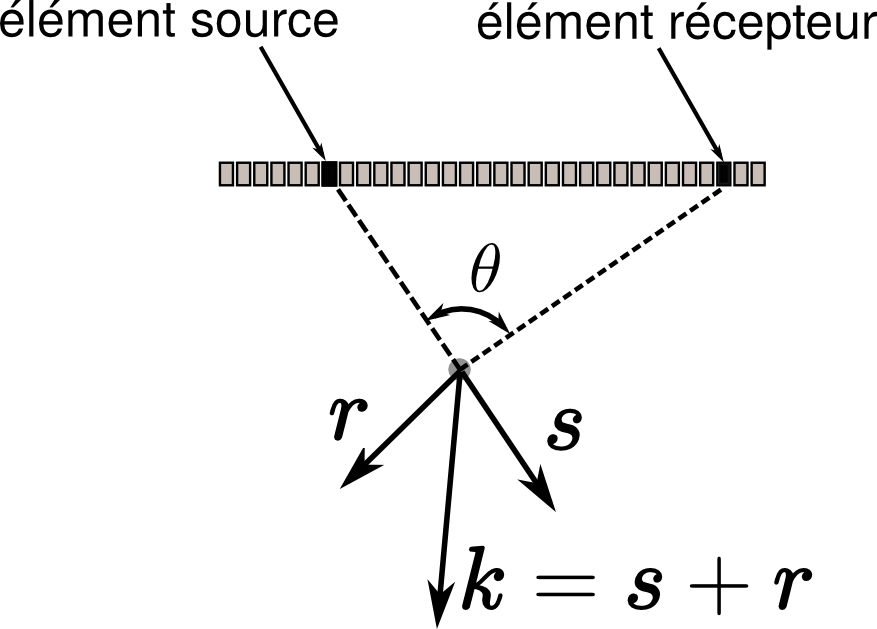
\includegraphics[height=3cm]{img/reso.png}
	\caption{Illustration de l'impact de l'angle de diffraction sur la résolution spatiale du gradient.\label{app:k1}}
\end{figure}


Une illustration du lien entre la couverture en nombres d'onde du milieu et l'acquisition ainsi que les sources miroirs est réalisée ci-après. Pour différentes configurations, des transformées de Fourier spatiales du gradient sont réalisées au niveau de 18 points diffractant, le paramètre du modèle étant la vitesse verticale (cf figure~\ref{app:config_reso}).

\begin{figure}[!h]
	\centering
	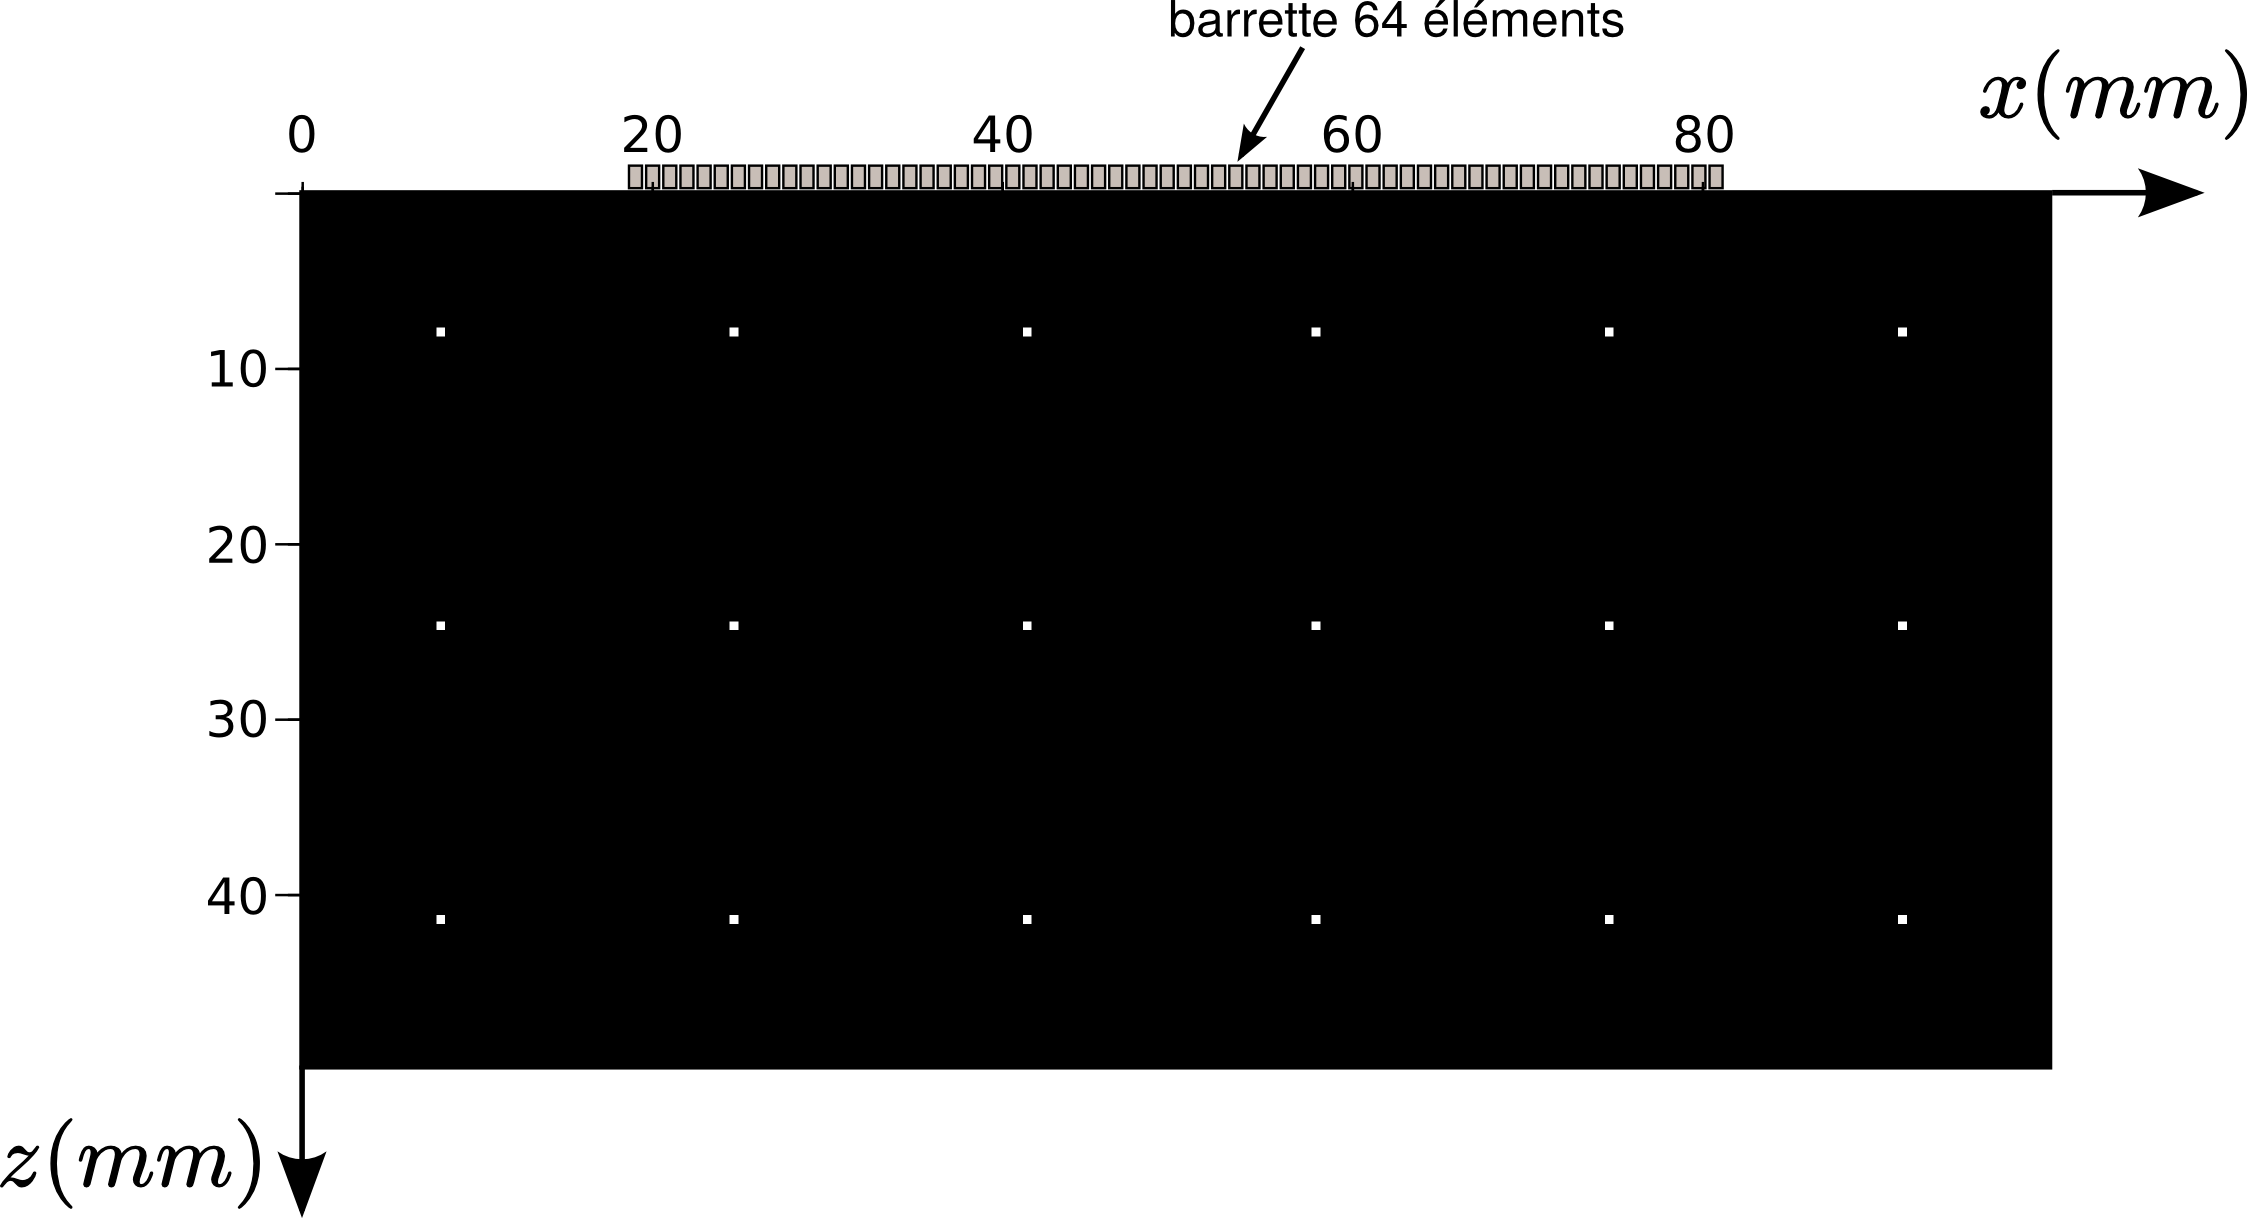
\includegraphics[height=5cm]{img/vp_scat.png}
	\caption{Configuration pour l'étude de résolution. La vitesse dans les inclusions est de 3000 m/s et de 6000 m/s ailleurs. Les éléments du transducteurs sont tous utilisés en réception et en transmission. \label{app:config_reso}}
\end{figure}


\subsection{Influence de la fréquence d'excitation}

Dans un premier temps, le milieu est entouré de conditions absorbantes. Les figures~\ref{app:150k} et~\ref{app:2M} montrent la couverture en nombres d'onde obtenue dans une configuration avec une barrette excitatrice et pour deux gammes de fréquence différentes. 
    
\begin{figure}[!h]
    \centering
    \begin{subfigure}[b]{0.05\textwidth}
 		\hspace{-2cm}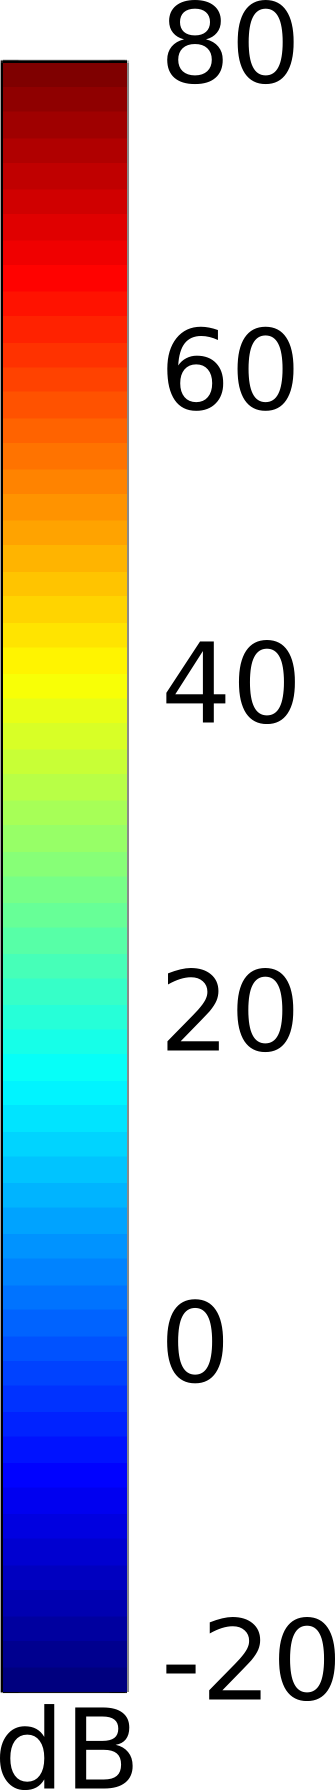
\includegraphics[width=0.5cm]{img/echelle_fft.png}\vspace{2.1cm}
	\end{subfigure}
    \begin{subfigure}[b]{0.4\textwidth}
		\hspace{-3cm}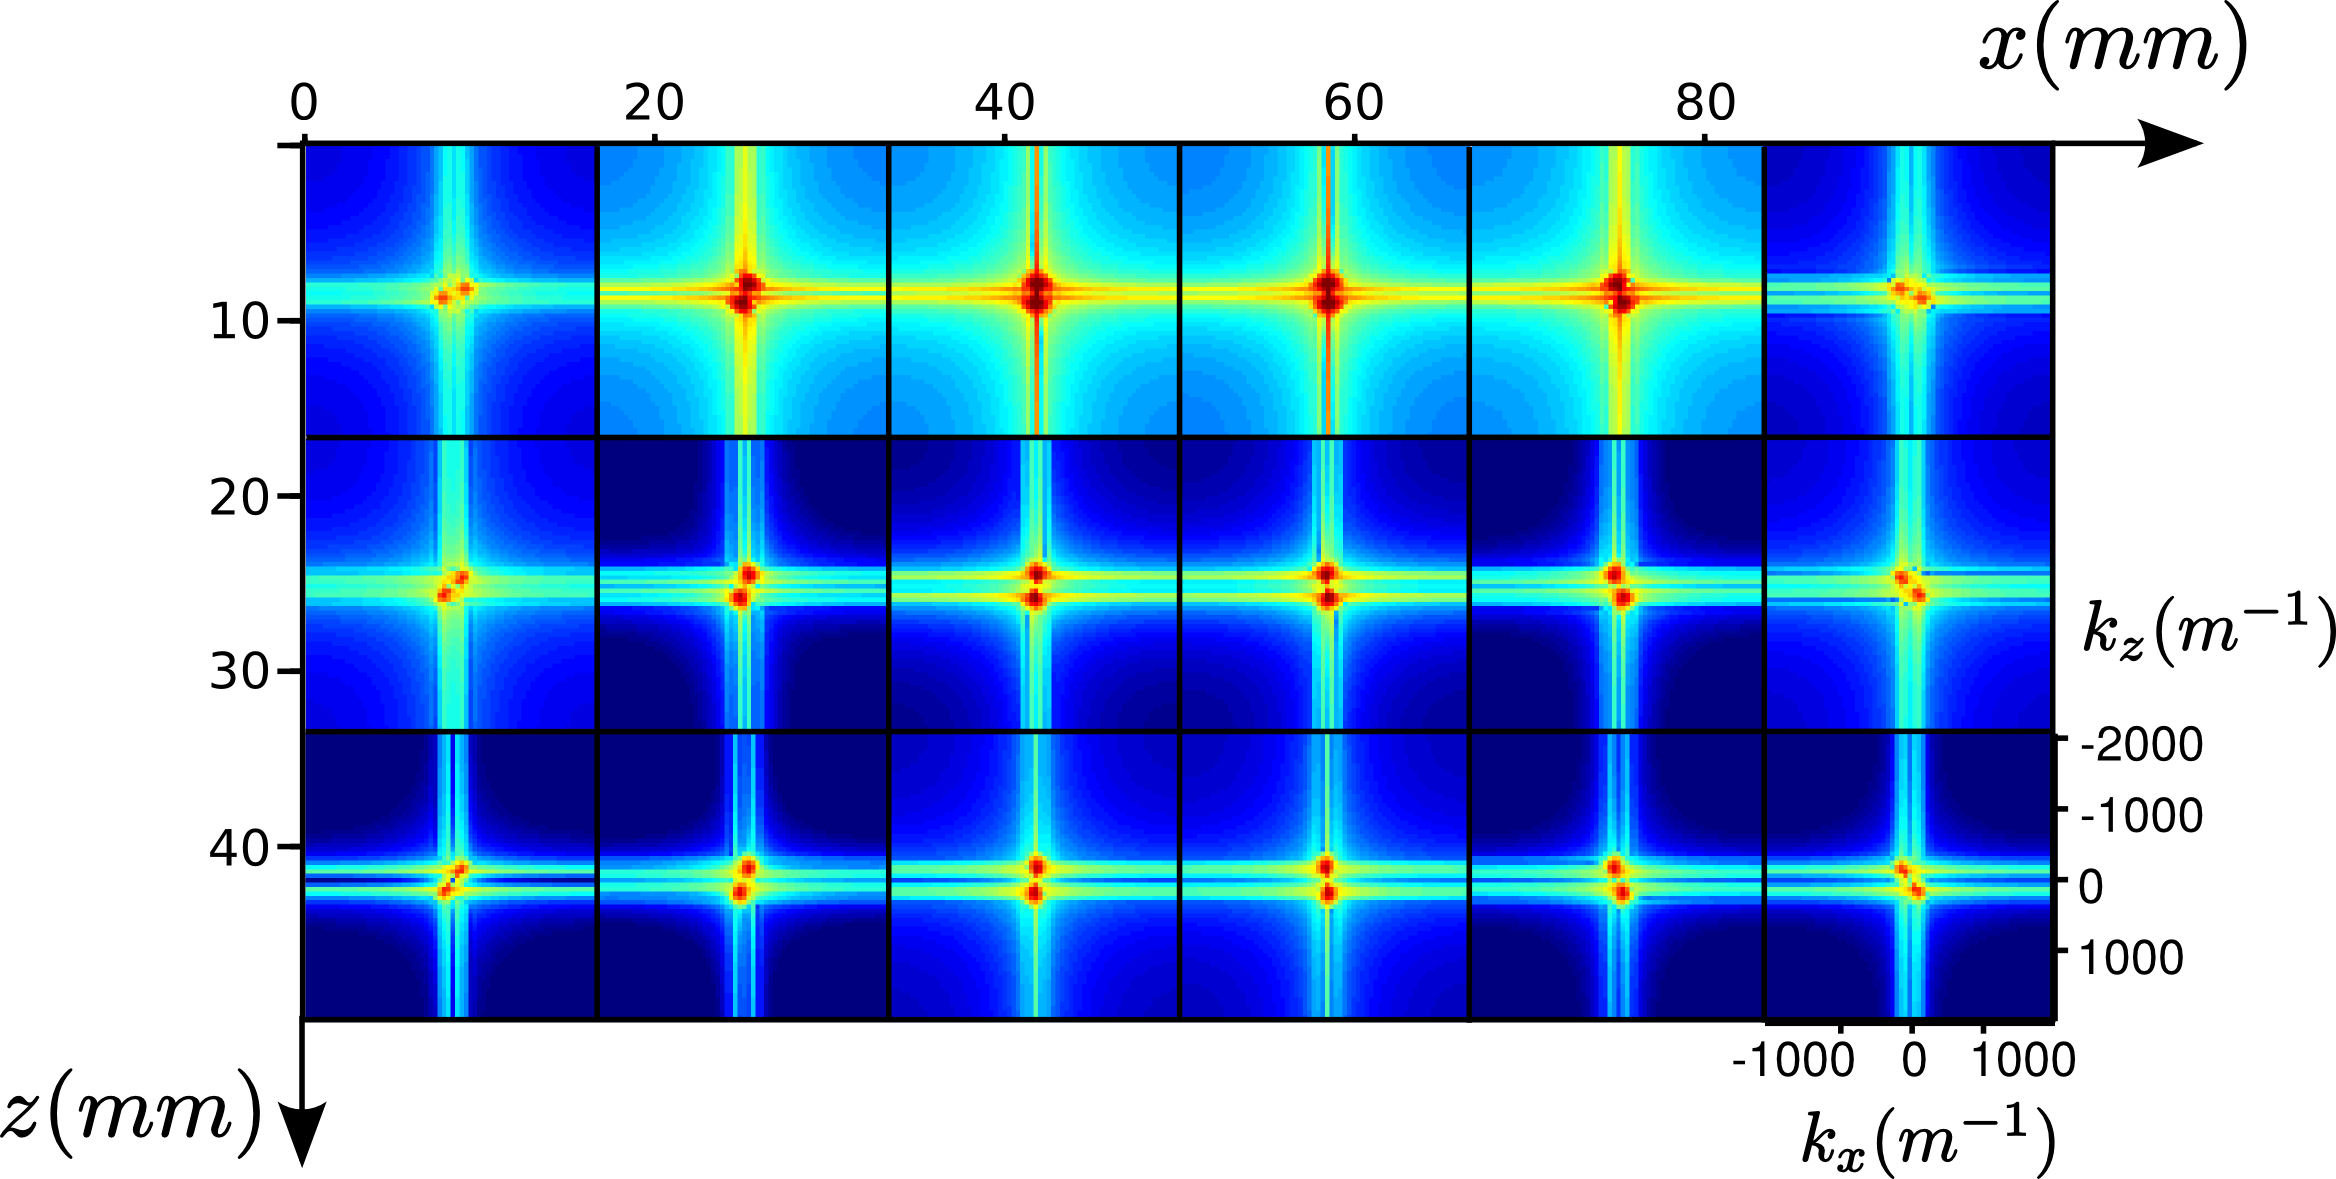
\includegraphics[width=1.5\textwidth]{img/ssfreesurf_150k}
		\caption{Excitation centrée à 150 kHz.}
		\label{app:150k}
	\end{subfigure}	
	%\hspace{0.7cm}
	\begin{subfigure}[b]{0.4\textwidth}
		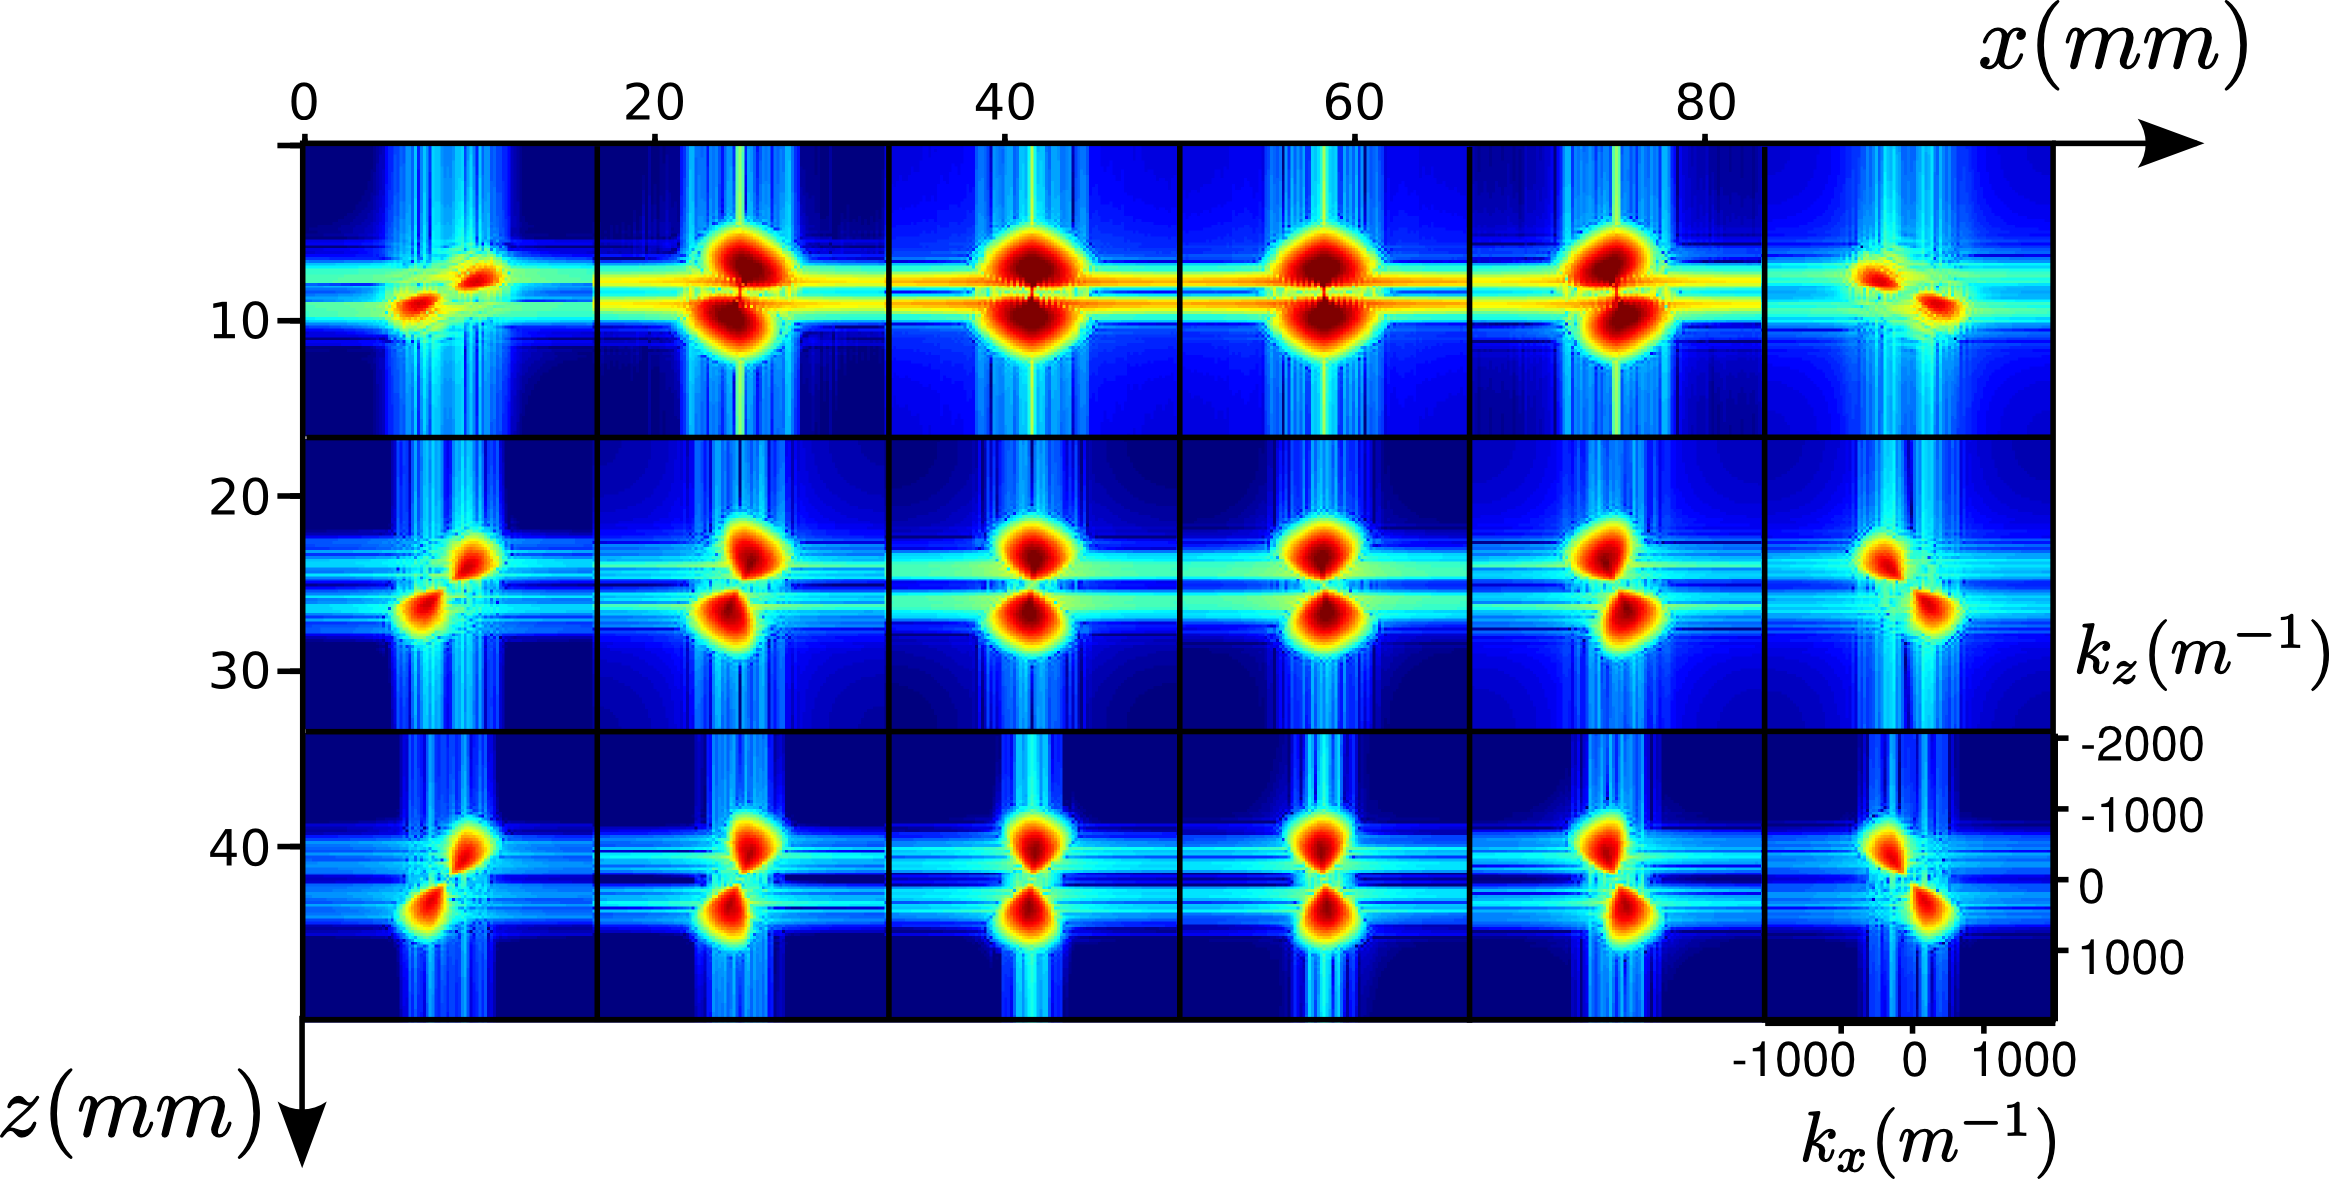
\includegraphics[width=1.5\textwidth]{img/fft2d_nofreesurf_2MHz.png}
		\caption{Excitation centrée à 2 MHz.}
		\label{app:2M}
	\end{subfigure}
	\caption{Transformées de Fourier spatiales locales pour 2 gammes de fréquence d'excitation.}
\end{figure}

Comme l'indique l'expression de $k$ (équation~\ref{app:nb_onde}), pour une excitation basse fréquence, le gradient est pauvre en hauts nombres d'onde. Inversement, l'excitation haute fréquence ne permet pas de reconstruire les bas nombres d'onde.\\
La couverture en nombre d'onde est également très liée à l'acquisition. Elle est meilleure aux abords et en direction de la barrette. Les nombres d'onde verticaux seront globalement mieux reconstruits avec cette acquisition qui favorise les petits angles de diffraction, tandis que la couverture en nombres d'ondes horizontaux est très faible.

\subsection{Influence des surfaces libres}

Deux surfaces libres sont maintenant ajoutées à la soudure de référence et au modèle initial. L'objectif est d'illustrer l'influence de la longueur du signal d'acquisition, soit le nombre de réflexions dans la plaques prises en compte dans les données. Les figures~\ref{app:1400pt} et~\ref{app:4200pt} montrent la couverture en nombres d'onde obtenue  pour 1 et 6 réflexions dans la plaque, pour une excitation à 2 MHz.

\begin{figure}[!h]
    \centering
    \begin{subfigure}[b]{0.05\textwidth}
 		\hspace{-2cm}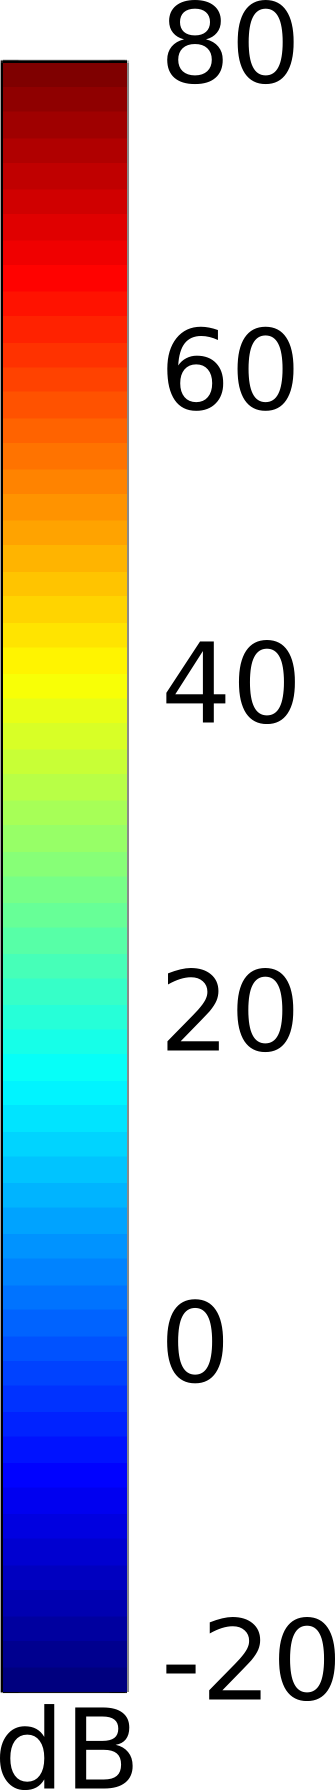
\includegraphics[width=0.5cm]{img/echelle_fft.png}\vspace{2.1cm}
	\end{subfigure}
    \begin{subfigure}[b]{0.4\textwidth}
		\hspace{-3cm}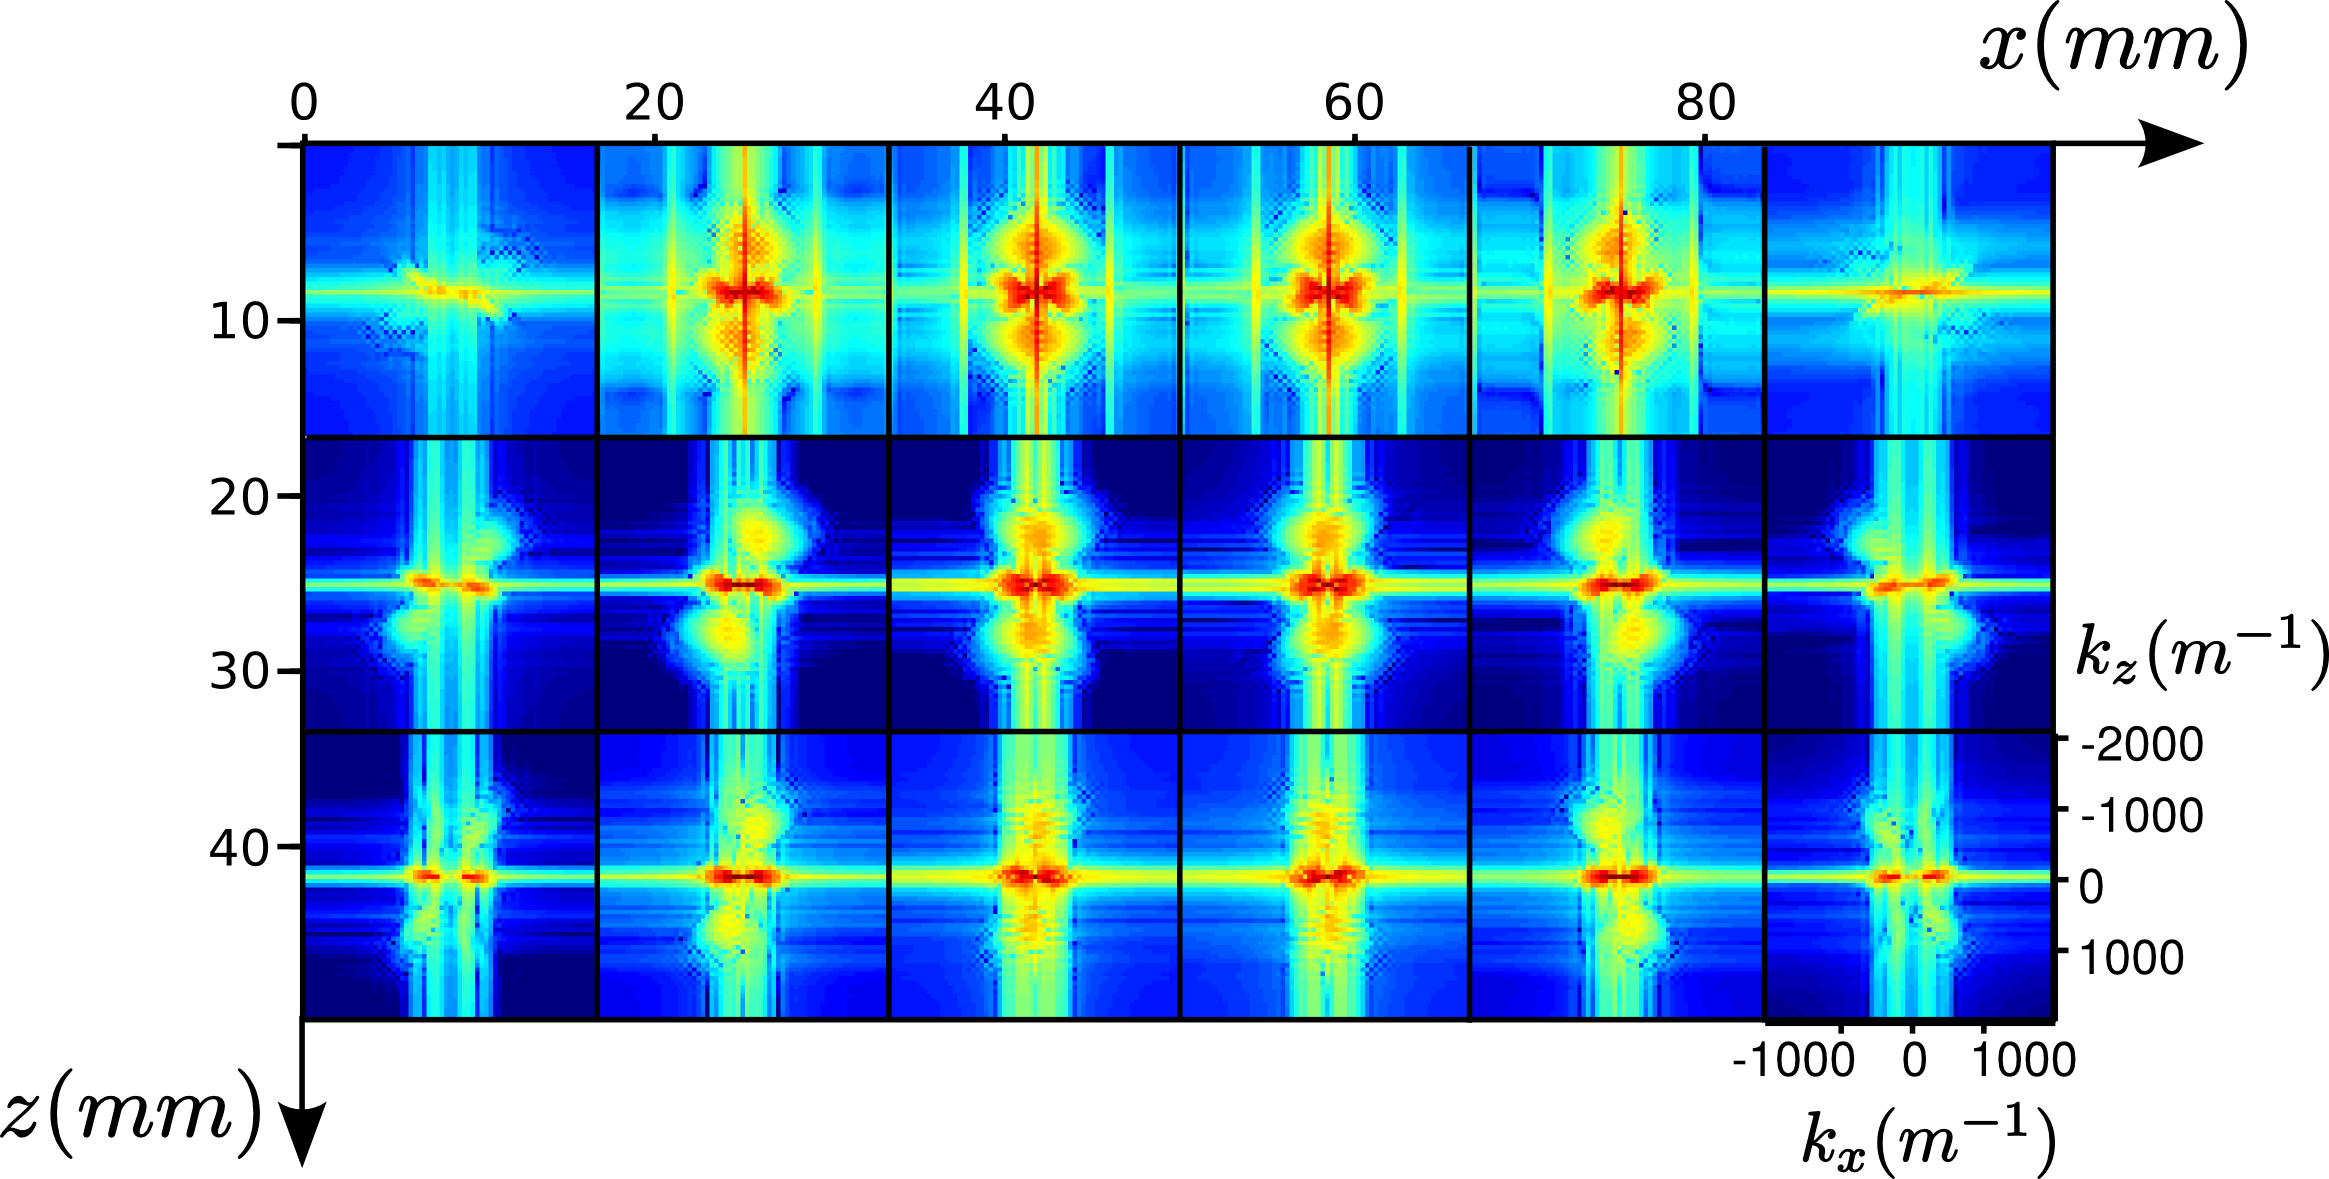
\includegraphics[width=1.5\textwidth]{img/1400pt.png}
		\caption{Pour une réflexion, soit un trajet de 1 aller-retour dans l'épaisseur de la plaque.}
		\label{app:1400pt}
	\end{subfigure}	
	\hspace{0.7cm}
	\begin{subfigure}[b]{0.4\textwidth}
		\hspace{-0.7cm}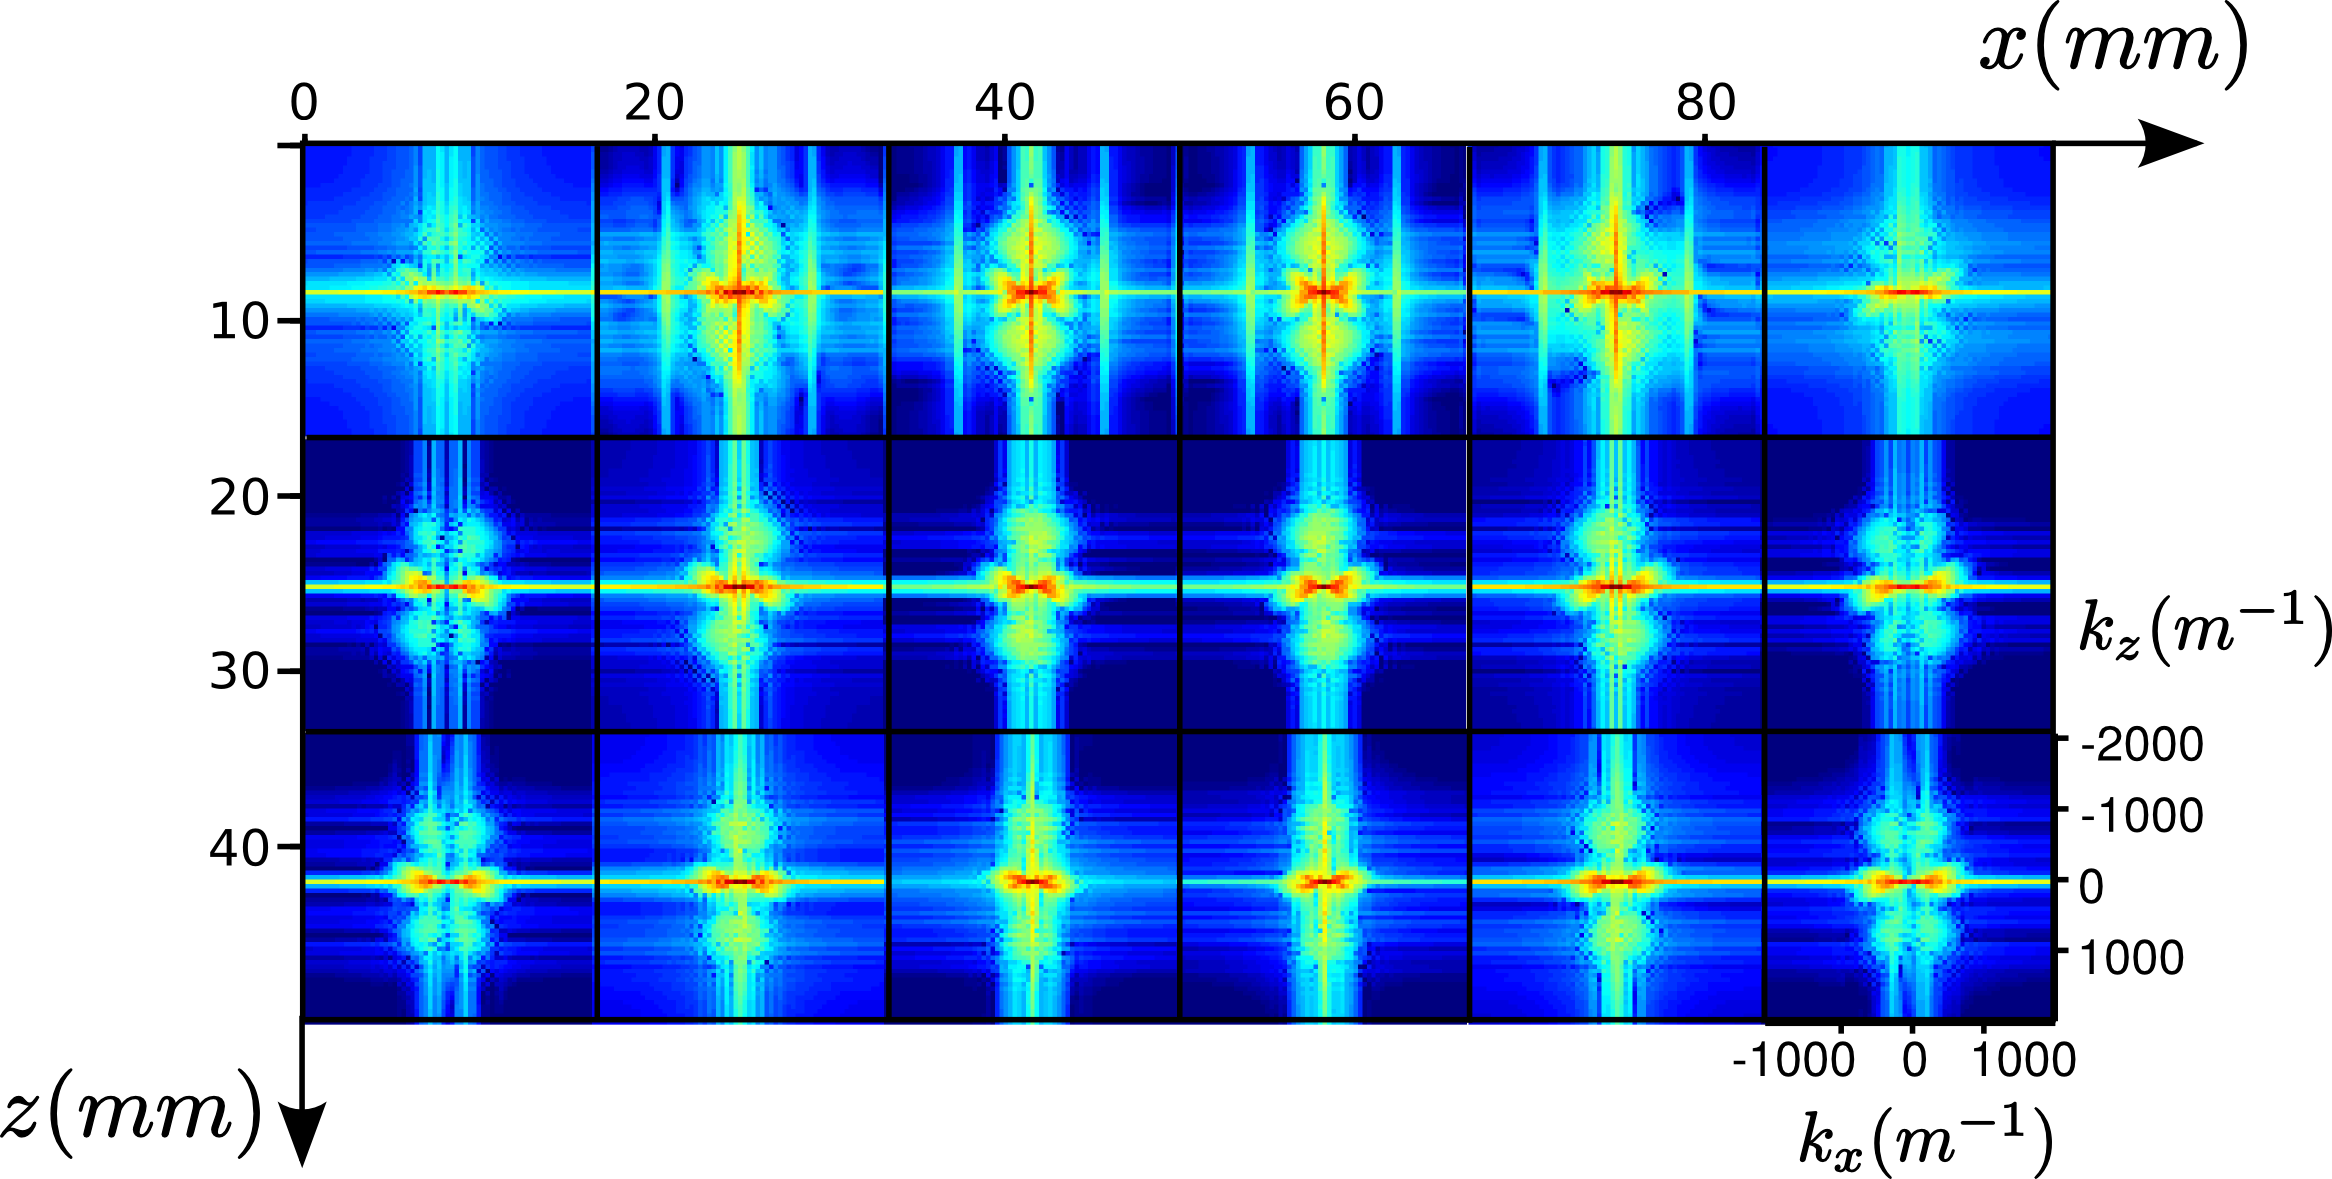
\includegraphics[width=1.5\textwidth]{img/4200pt.png}
		\caption{Pour 6 réflexions, soit un trajet de 3 aller-retours dans l'épaisseur de la plaque.}
		\label{app:4200pt}
	\end{subfigure}
	\caption{Transformées de Fourier spatiales locales du gradient pour 2 durées d'acquisition. La fréquence d'excitation est centrée à 2 MHz.}
\end{figure}

Les surfaces libres sont assimilables à l'ajout de sources images éloignées qui favorisent une propagation verticale et de grands angles de diffraction (figure~\ref{app:reso_surf_libre}). Ainsi, les nombres d'onde horizontaux sont beaucoup mieux couverts avec, en contrepartie, une perte sur les nombres d'onde verticaux.  \\
Lorsque 6 réflexions sont prises en compte, l'ensemble des nombres d'ondes purement horizontaux est reconstruit, mais la résolution verticale est presque nulle.
\begin{figure}[!h]
	\centering
	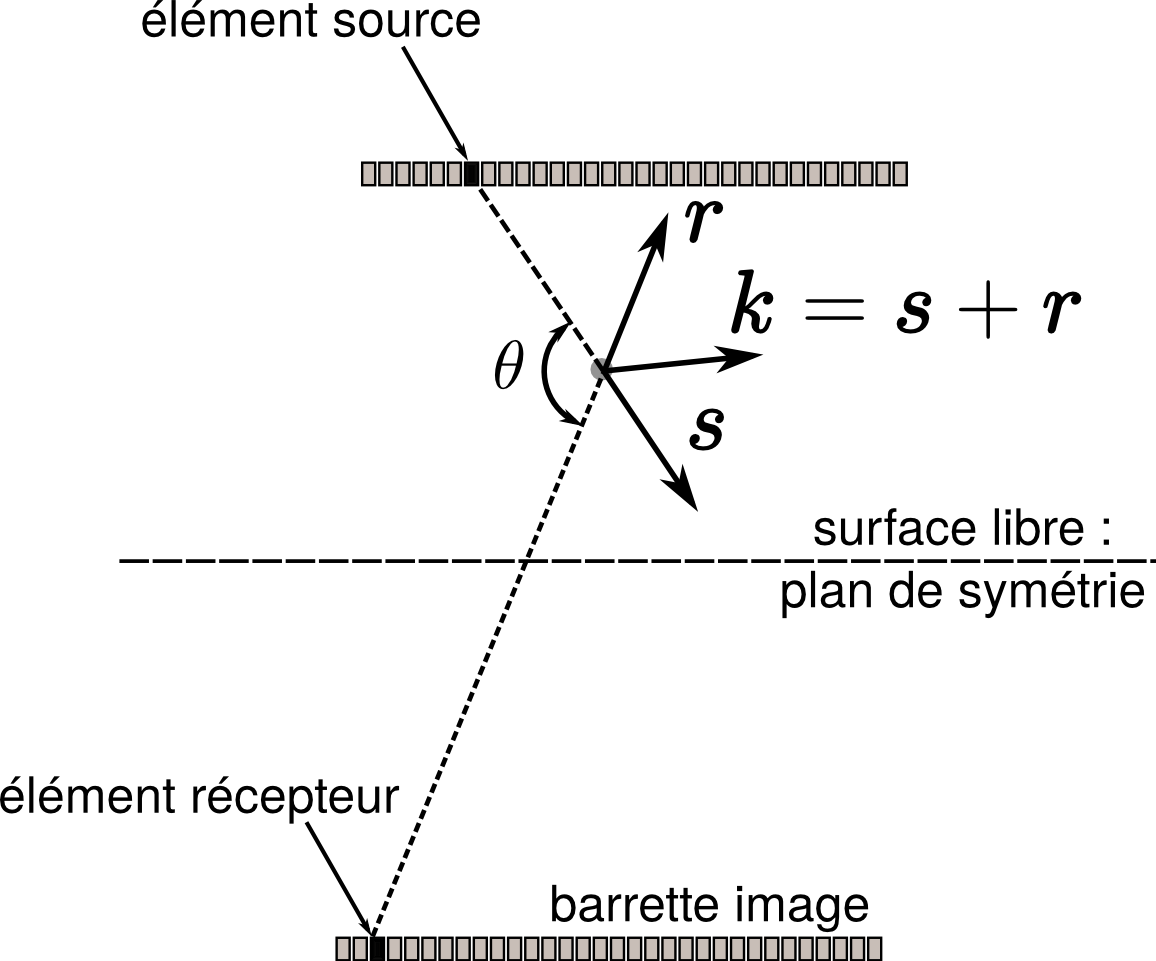
\includegraphics[height=5cm]{img/reso_surf_libre.png}
	\caption{Illustration de l'impact d'une surface libre sur la résolution spatiale du gradient : la propagation verticale est favorisée, ainsi que les grands angles de diffraction.\label{app:reso_surf_libre}}
\end{figure}



Finalement, la prise en compte d'une réflexion dans les données d'acquisition permet d'améliorer la reconstruction des nombres d'onde horizontaux et donc la résolution latérale des défauts, tout en assurant une bonne couverture en nombres d'onde verticaux.


\section{Gestion des non-linéarités}
Une stratégie pour limiter la non-linéarité de l'inversion consiste à réaliser l'inversion en plusieurs temps, en injectant progressivement le contenu haute fréquence dans les données. L'inversion à basse fréquence permet ainsi de reconstruire la structure grossière avant d'ajouter les détails grâce à la résolution qu'offre le gradient en haute fréquence.\\



Afin que les nombres imagés soient correctement échantillonnés, il faut que le plus grand nombre d'onde imagé à une fréquence soit le même que que le plus petit à la fréquence suivante \citep{sirgue}. En considérant que le plus nombre d'onde est obtenu pour une angle de diffraction de $\pi/2$ , le rapport de fréquences suivant doit donc être respecté : 

\begin{alignat*}{3}
	  ~&k_{max}(f_{n}) &&= k_{min}(f_{n+1})\\
	\Leftrightarrow~~~~~ &  f_n &&= f_{n+1}\cos \left(\frac{\pi}{2} \right)\\
	 \Leftrightarrow~~~~~ & \frac{f_{n+1}}{f_n} && \approx  1,5.
\end{alignat*} 

Les inversions présentées ci-après sont donc réalisées en plusieurs itérations. Entre chaque itérations, les données observées et l'ondelette d'excitation sont filtrées par un filtre passe-bas de fréquence centrale $f_{n}$ et dont la fréquence de coupure haute est de $2,5 \times f_{n}$.


\section{Inversions en milieu acoustique}

Dans un premier temps, la méthode d'imagerie est appliquée à des milieux acoustiques, ce qui simplifie le problème et réduit les coût de calcul. Le code utilisé est \emph{TOYxDacTIME} développé dans le cadre du projet \emph{Seiscope}\footnote{http://seiscope2.osug.fr}. Le problème direct y est résolu par différences finies d'ordre 2.\\
%, ce qui impose deux contraintes de discrétisation : dispersion numérique, cfl 

La propagation des ondes élastiques est décrite par les équations linéarisées en déplacements $\bm{u}$ et contraintes $\bar{\bar T}$ suivantes \citep{mat_ac} : 

\begin{eqnarray}
	\rho \frac{\dd^2 u_{i}}{\dd t^2} &=& \displaystyle\sum_{j}\frac{\dd T_{ij}}{\dd x_{j}}\\
	T_{ij}&=&C_{ijkl}\left( \frac{\dd u_{i}}{\dd x_{j}} + \frac{\dd u_{j}}{\dd x_{i}}\right)\text{,}
	\label{prop}
\end{eqnarray}
avec $C_{ijkl}$ le tenseur des constantes élastiques. Les études en milieu acoustique sont menées en approximation 2D : on suppose que le problème ne dépend pas de la dimension données par $\bm{\overrightarrow{x_3}}$.\\

Les équations de la propagation acoustique peuvent être déduite de~\ref{prop} en considérant un module de cisaillement nul. on a alors $T_{ij}=0$ si $i\neq j$.

\subsection{Isotrope}
On considère, tout d'abord, une propagation dans un milieu acoustique isotrope. Les constantes élastiques sont alors égales dans toutes les directions et les propriétés élastiques sont donc réduites à une seule constante. Les équations~\ref{prop} deviennent : 
\begin{eqnarray}
	\rho \frac{\dd^2 u_{i}}{\dd t^2} = -\bm{\nabla} p\\
	p=-\kappa \displaystyle\sum_{i} \frac{\dd u_{i}}{\dd x_{i}}\text{,}
\end{eqnarray}
avec $\kappa$ le module de rigidité et $p$ la pression.

Les données observées sont calculées à partir du milieu dont la densité et  la vitesse verticale sont présentés en figure~\ref{app:iso:model}. On considère une configuration d'acquisition favorable à un bon éclairage de la soudure : deux barrettes de 64 éléments (en émission et réception) sont situées de part et d'autre de la soudure. Cette configuration ne correspond pas à celle d'une inspection de soudure conventionnelle, puisque en pratique, le relief de la soudure ne permet pas de placer les barrettes directement dessus.\\

\begin{figure}[!h]
	\centering
	\begin{subfigure}[b]{0.45\textwidth}
		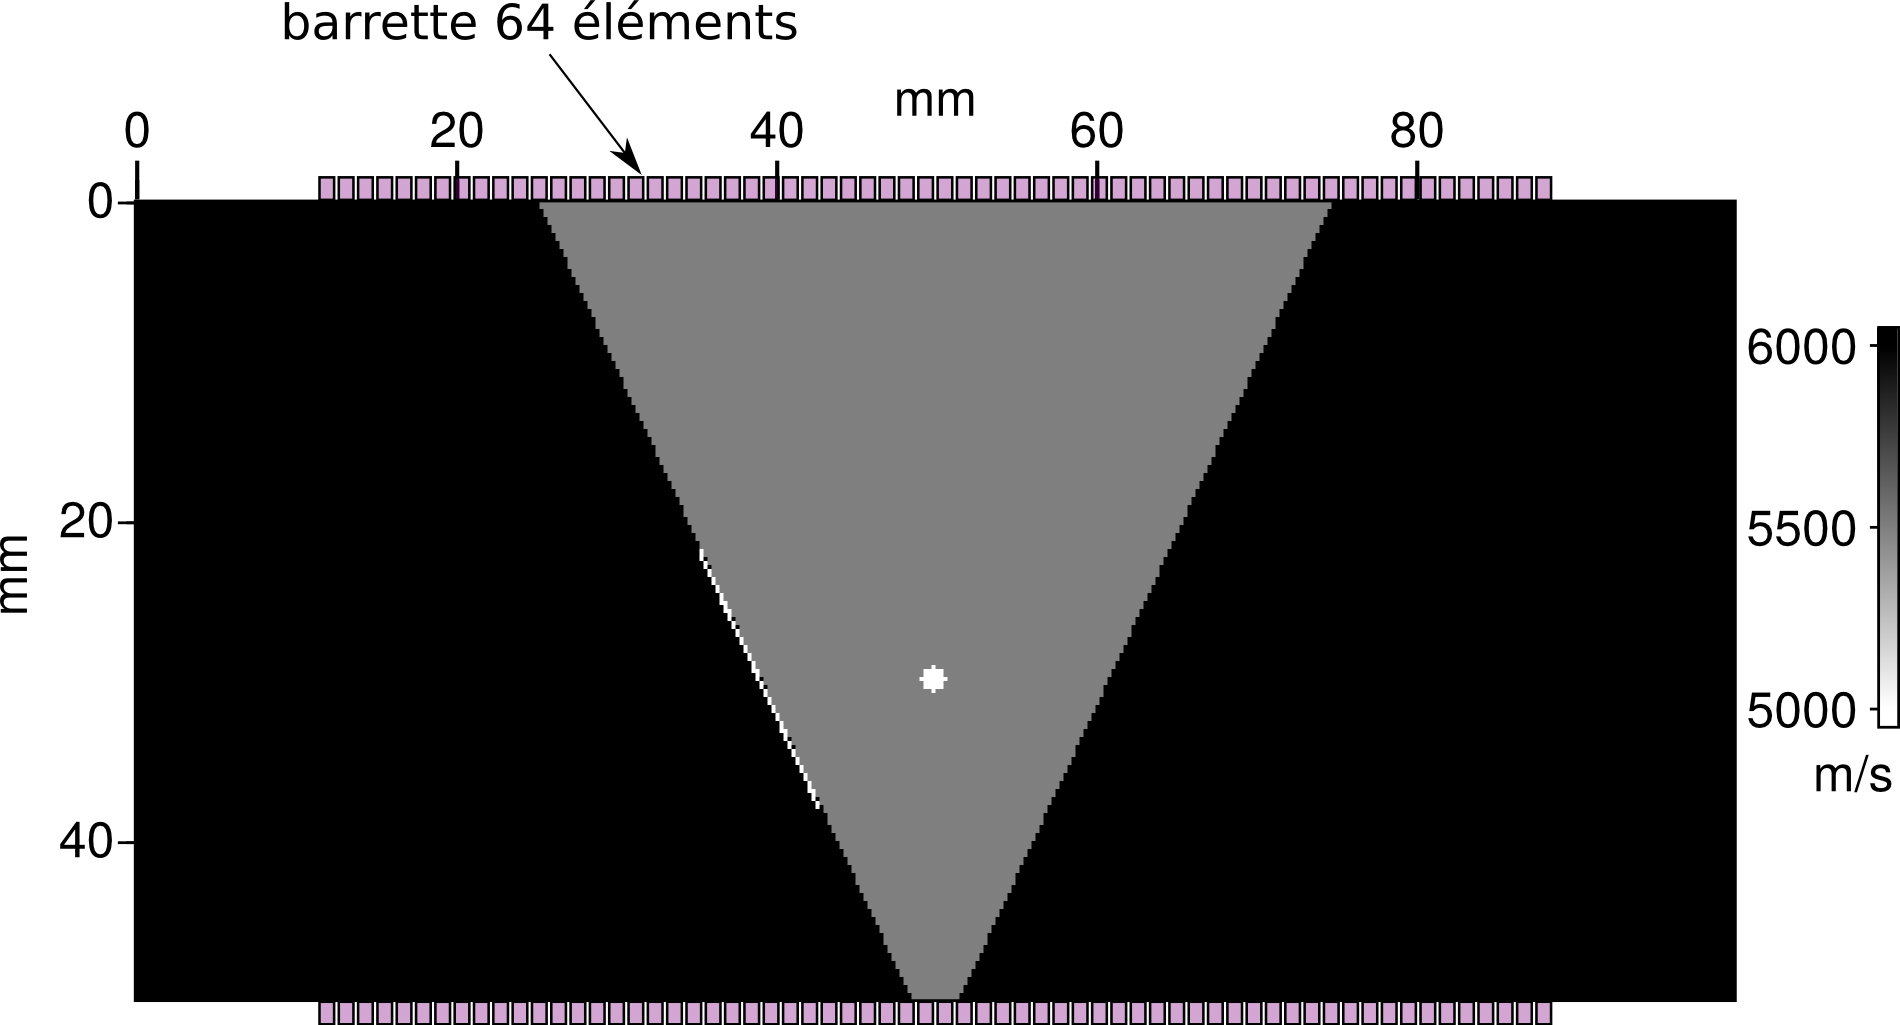
\includegraphics[width=\textwidth]{img/milieux_ps/vp_true.png}
		\caption{Vitesse vraie.}
	\end{subfigure}
	\begin{subfigure}[b]{0.45\textwidth}
		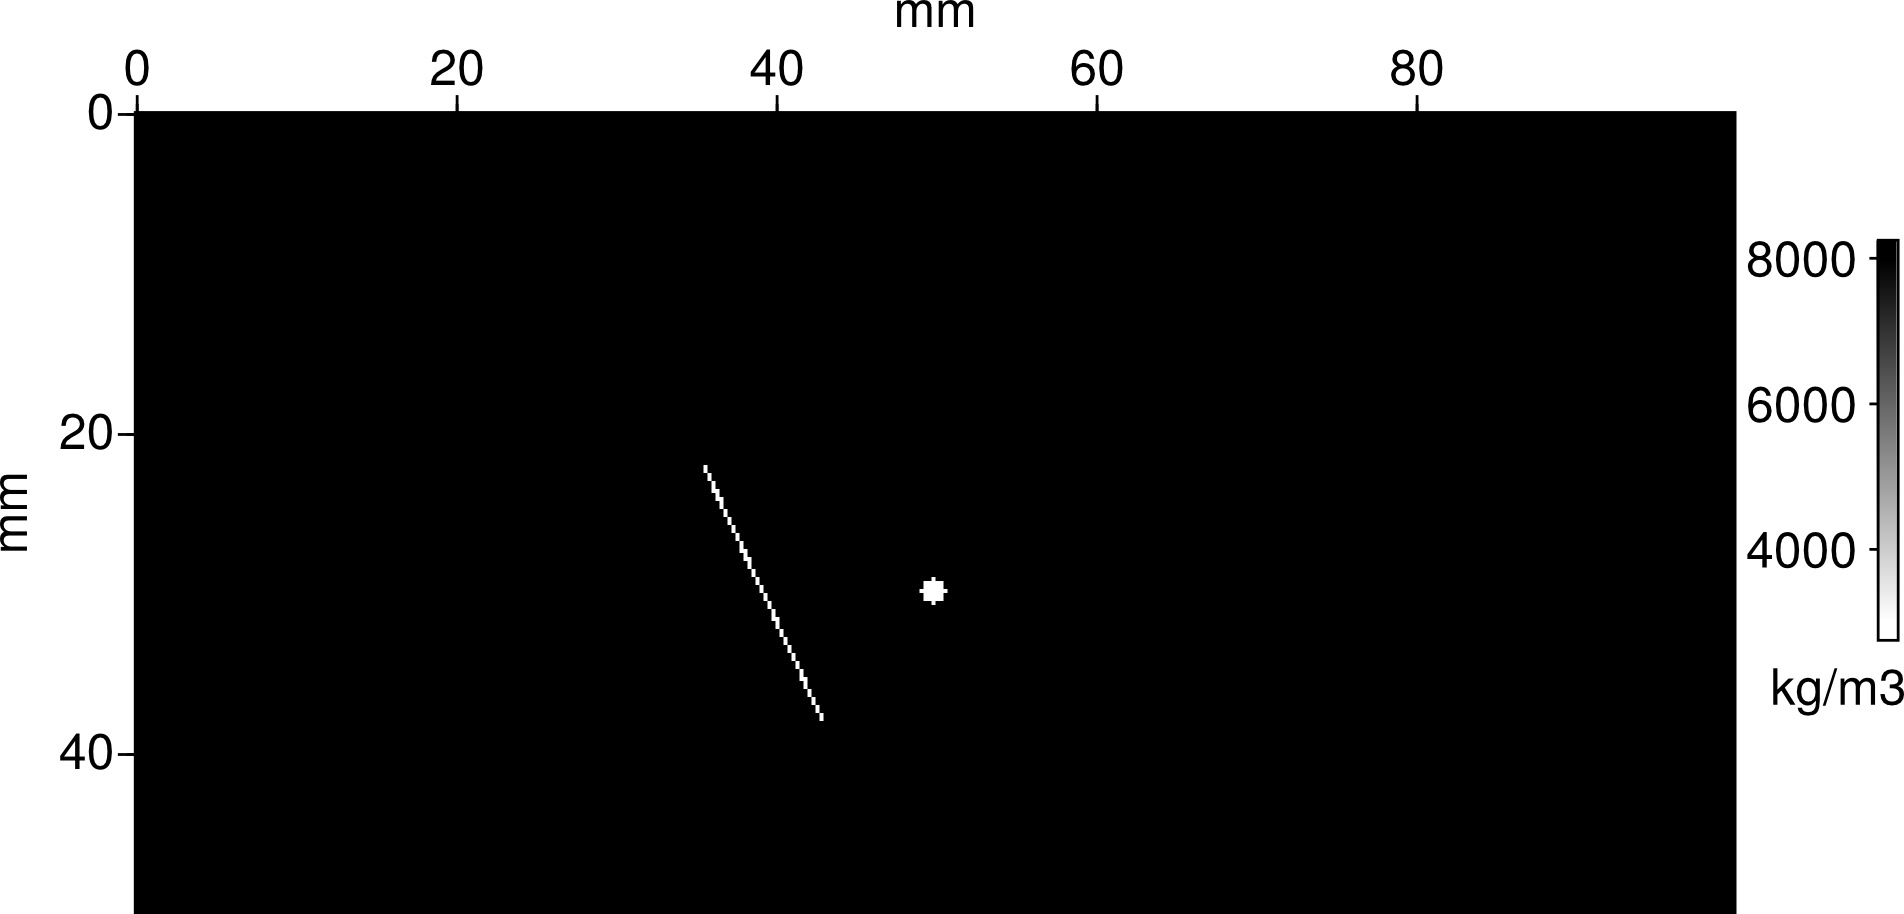
\includegraphics[width=\textwidth]{img/milieux_ps/rho_true.png}
		\caption{Masse volumique vraie.}
	\end{subfigure}
	\caption{Milieux en vitesse et masse volumique pour la génération des données observées. Deux barrettes de 64 éléments sont utilisées en réception et en transmission, de part et d'autre de la soudure. La soudure simulée présente deux défauts : une inclusion de diamètre $\lambda/2$ et un manque de fusion de largeur $\lambda/12$.\label{app:iso:model}}
\end{figure}

%Les modèles initiaux pour l'inversion sont uniformes, avec $v_{p}=6000$~m/s et $\rho=8000$~kg/m$^3$.

\subsubsection{Inversions monoparamètres}

Une première inversion est réalisée, en gardant $\rho$ à sa valeur initiale et en ne mettant à jour que le modèle de vitesse, pour 9 bandes de fréquences allant de 100 kHz à 3,4 MHz. Le modèle initial de vitesse pour cette inversion est pris uniforme avec $v_{p}=6000$~m/s.\\

Une seconde inversion monoparamètre est proposée pour une reconstruction de la masse volumique. Cependant, il est très difficile d'assurer une convergence en prenant des modèles initiaux de vitesse et de densité uniformes, car la seule mise à jour du modèle de densité ne peut expliquer la majeure partie des données en terme de cinématique. En effet, la figure~\ref{app:traces_rho} montre que la différence de densité au niveau des défauts n'impacte pas les temps de vol mais l'amplitude des diffractions sur les défauts. Il est donc nécessaire de disposer d'un modèle de vitesse suffisamment précis pour expliquer les différentes arrivées, puis la densité sera reconstruite par correction des amplitudes. La vitesse initiale utilisée pour cette inversion est issue d'une première inversion de la vitesse avec une régularisation forçant fortement le lissage de la reconstruction.\\

Enfin, une troisième inversion de la vitesse est réalisée, avec pour modèle initial ce même modèle de vitesse lissé.

Les modèles initiaux de vitesse et le résultats de ces inversions se trouvent figure~\ref{app:inv_mono}. 
\todo[inline]{commenter résultat : influence du rayonnement \\
même à basse fréquence, on introduit des artefacts haute fréquence}

\begin{figure}[!h]
	\centering
	\begin{subfigure}[b]{0.45\textwidth}
		\centering
		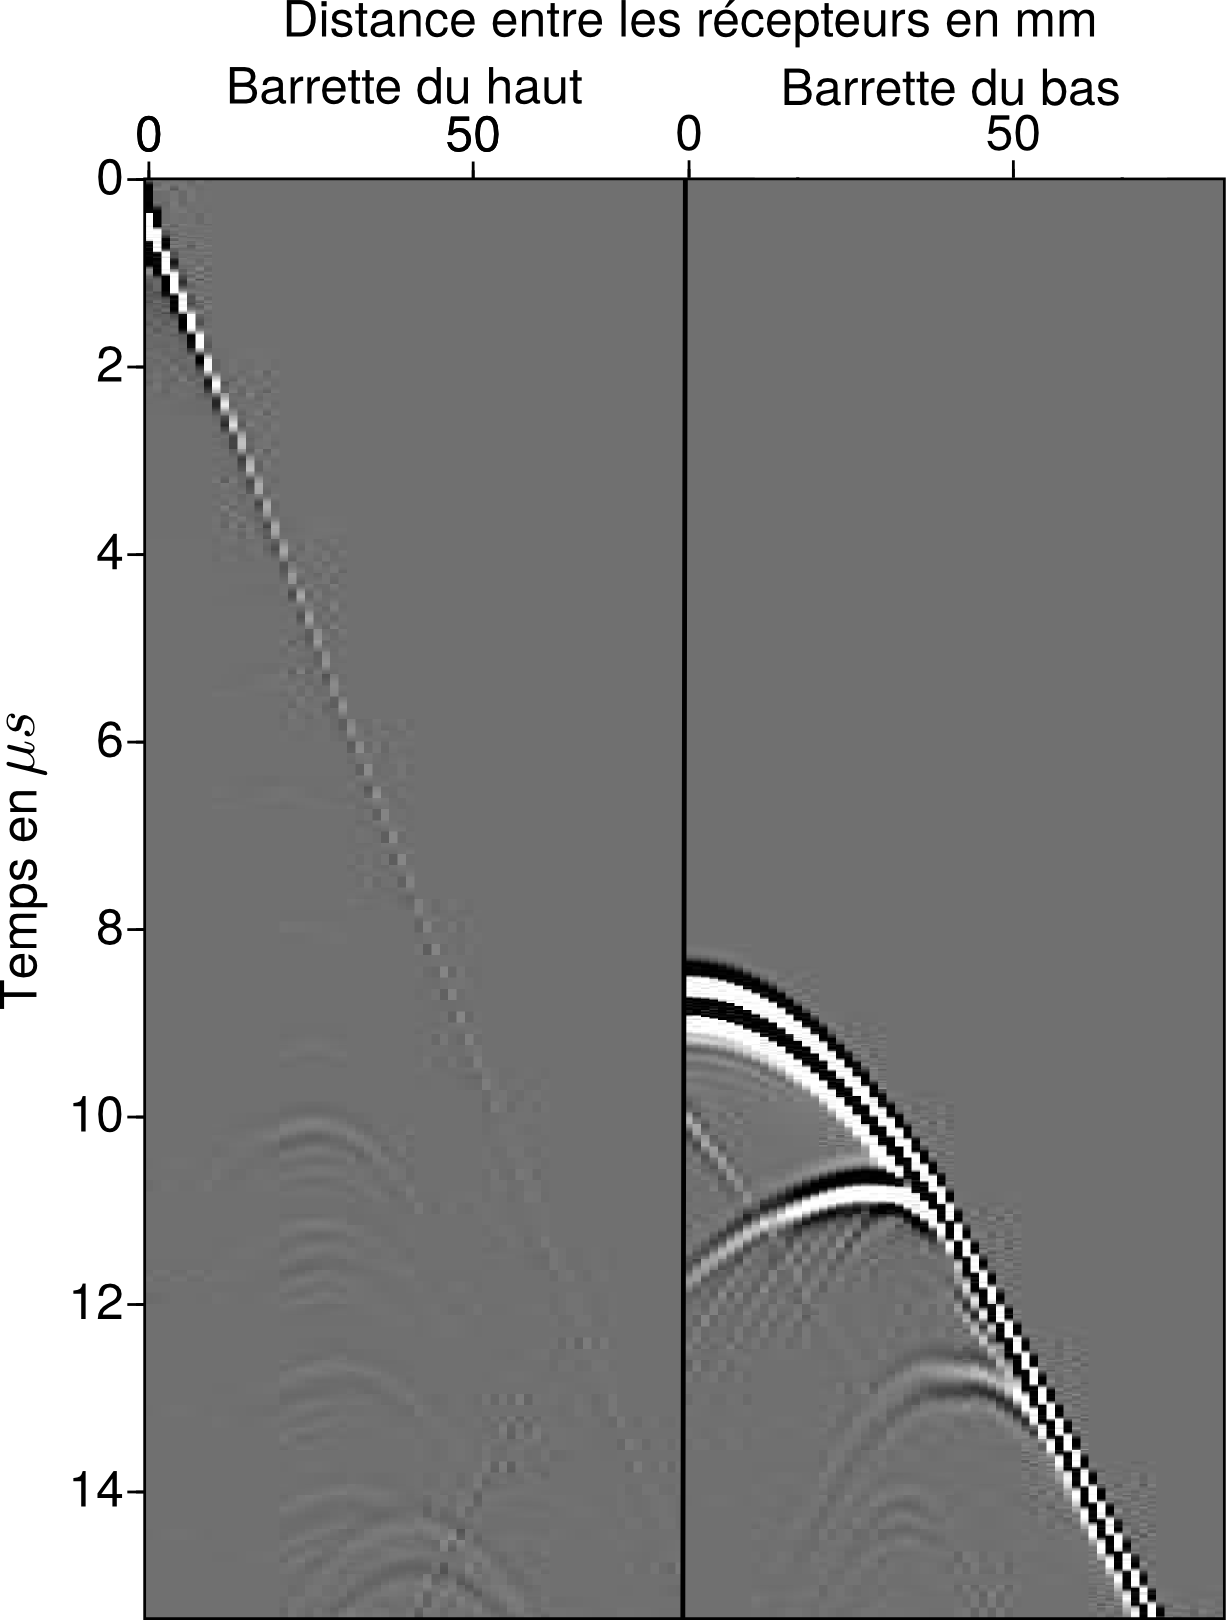
\includegraphics[width=0.8\textwidth]{img/rho_sur_donnees/data_rho_uni.png}
		\caption{Pour une densité uniforme.}
	\end{subfigure}
		\begin{subfigure}[b]{0.45\textwidth}
		\centering
		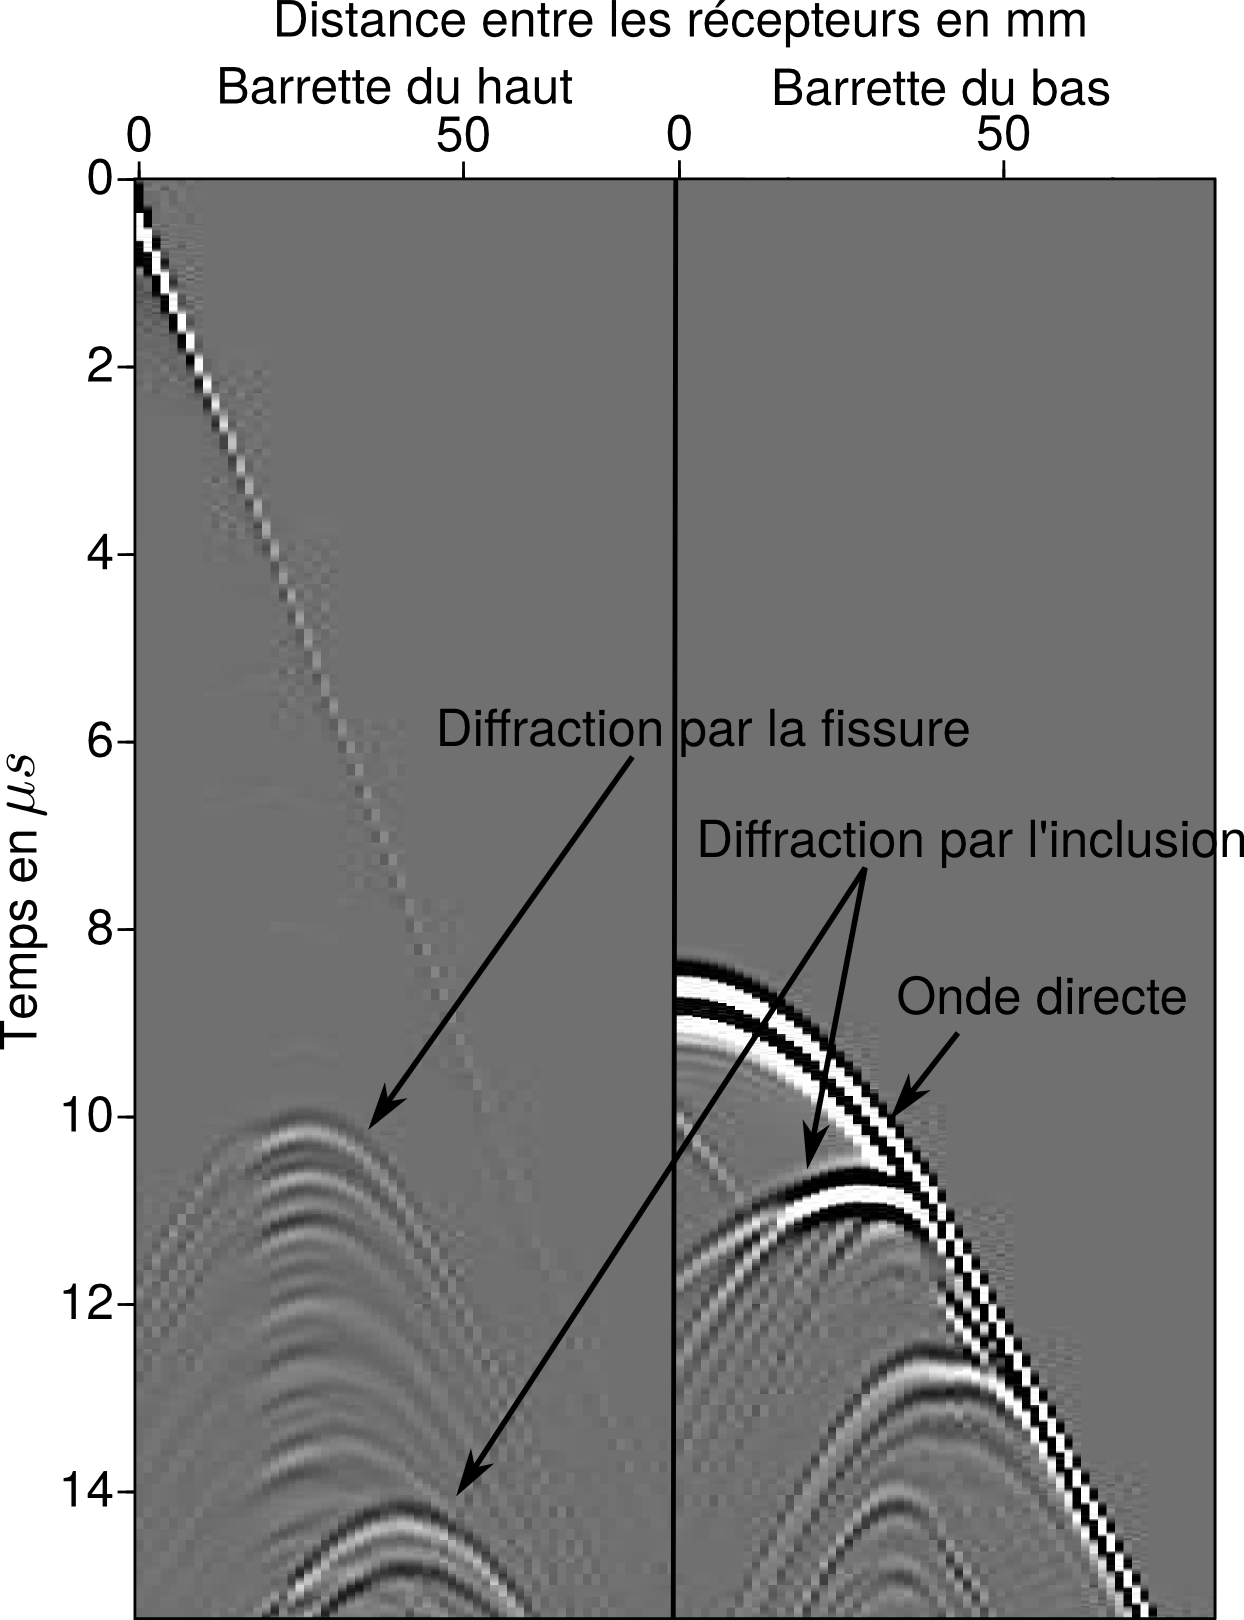
\includegraphics[width=0.8\textwidth]{img/rho_sur_donnees/data_rho_vrai.png}
		\caption{Pour $\rho=3000$~kg/m$^{3}$ dans les défauts.}
	\end{subfigure}
	\caption{Effet du contraste de densité sur les données observées (même échelle d'amplitude).\label{app:traces_rho}}	
\end{figure}



	\begin{figure}[!h]
	\begin{changemargin}{-2cm}{-2cm}
		\centering
		\begin{subfigure}[b]{0.29\textwidth}
			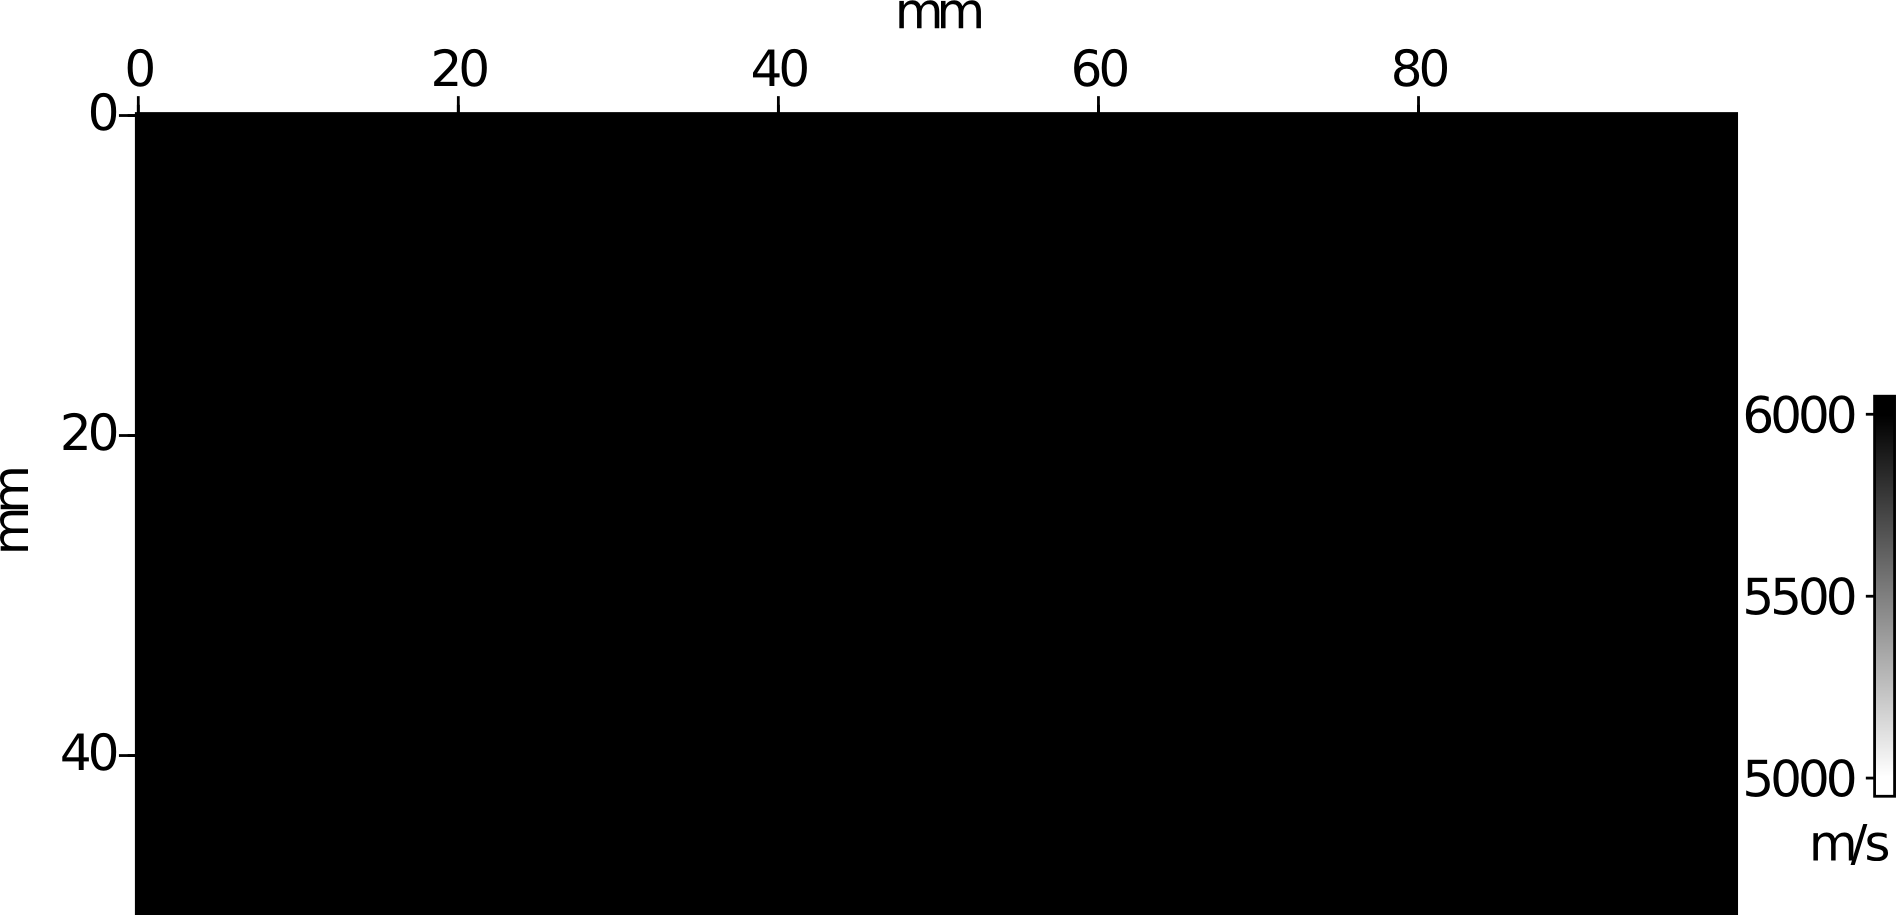
\includegraphics[width=\textwidth]{img/mono_param/vp_uni.png}
			\caption{Vitesse initiale pour l'inversion de la vitesse.}
		\end{subfigure}
		\begin{subfigure}[b]{0.29\textwidth}
			\includegraphics[width=\textwidth]{img/mono_param/vp_smooth.png}
			\caption{Vitesse initiale pour la seconde inversion de la vitesse.}
		\end{subfigure}
		\begin{subfigure}[b]{0.29\textwidth}
			\includegraphics[width=\textwidth]{img/mono_param/vp_smooth.png}
			\caption{Vitesse initiale pour l'inversion de la densité. }
		\end{subfigure}
		\begin{subfigure}[b]{0.29\textwidth}
			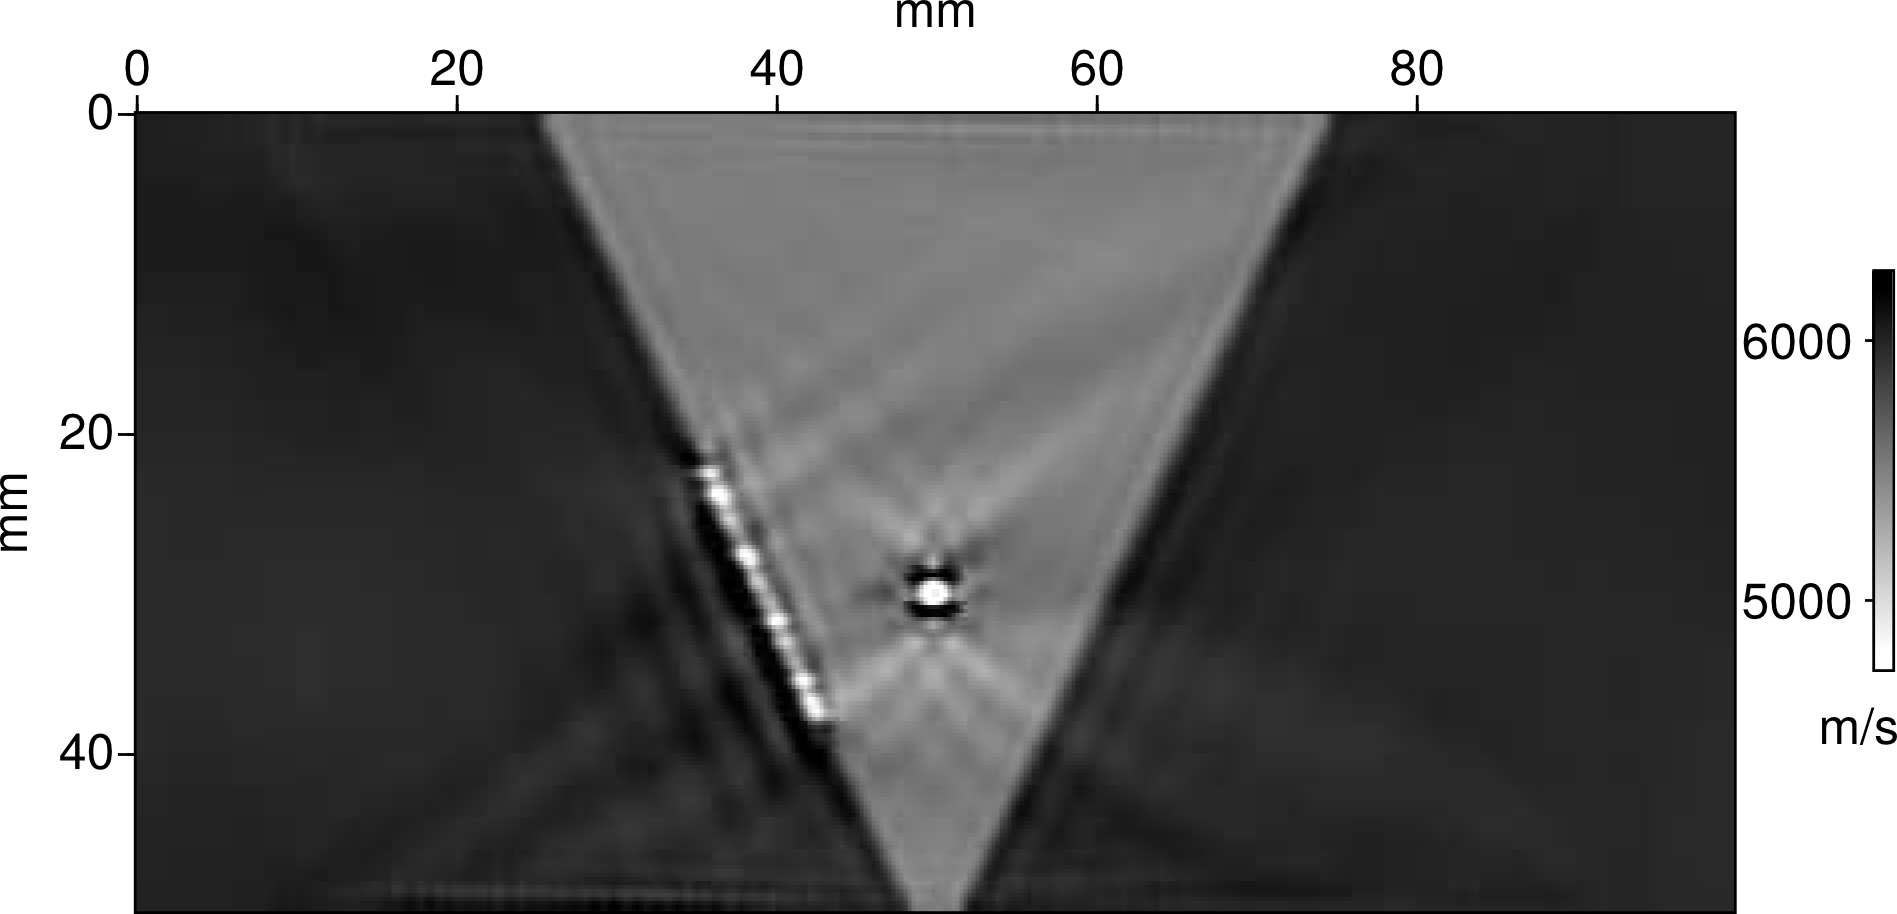
\includegraphics[width=\textwidth]{img/mono_param/vp_mono.png}
			\caption{Modèle final de vitesse obtenu par FWI monoparamètre.}
		\end{subfigure}
		\begin{subfigure}[b]{0.29\textwidth}
			%\includegraphics[width=\textwidth]{}
			\caption{.}
		\end{subfigure}
		\begin{subfigure}[b]{0.29\textwidth}
			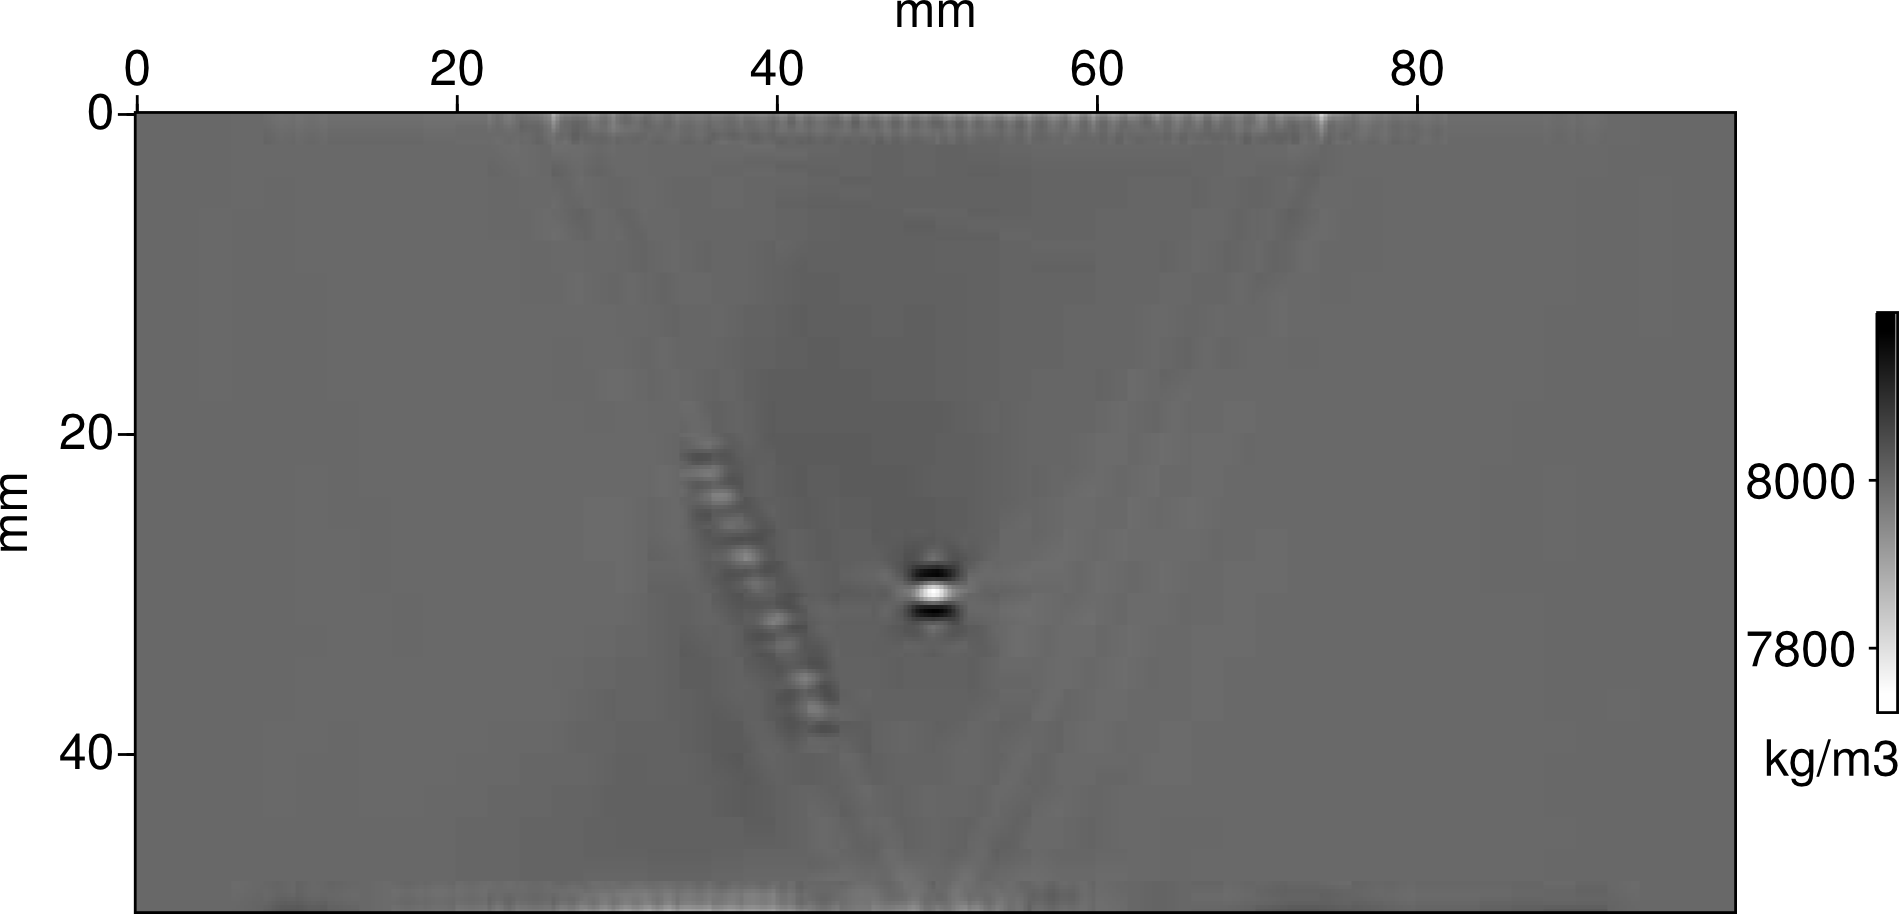
\includegraphics[width=\textwidth]{img/mono_param/rho_mono.png}
			\caption{Modèle final pour la densité obtenu par FWI monoparamètre. }
		\end{subfigure}
			\begin{subfigure}[b]{0.29\textwidth}
			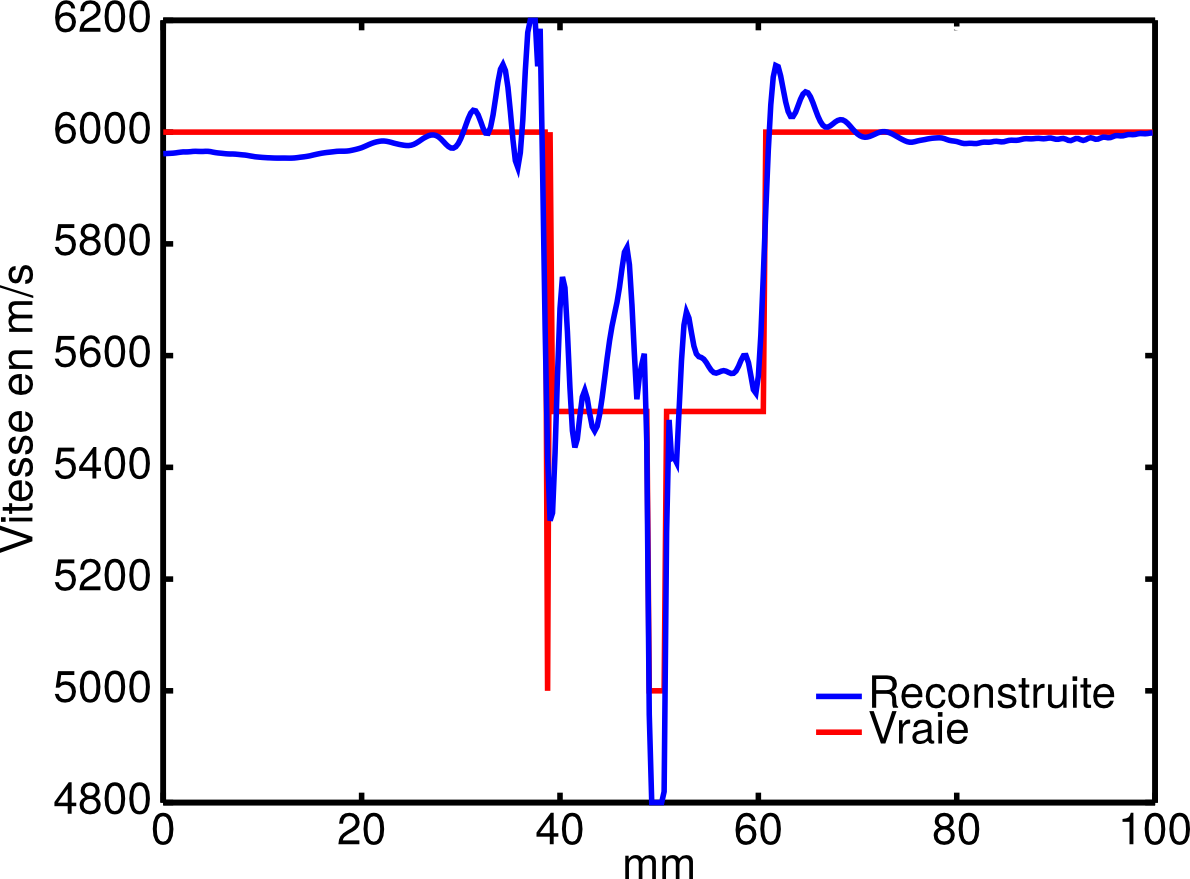
\includegraphics[width=\textwidth]{img/mono_param/coupe_vp_mono.png}
			\caption{Vitesses vraie et vitesse reconstruite à 3 cm de profondeur.}
		\end{subfigure}
		\begin{subfigure}[b]{0.29\textwidth}
			%\includegraphics[width=\textwidth]{}
			\caption{ }
		\end{subfigure}
		\begin{subfigure}[b]{0.29\textwidth}
			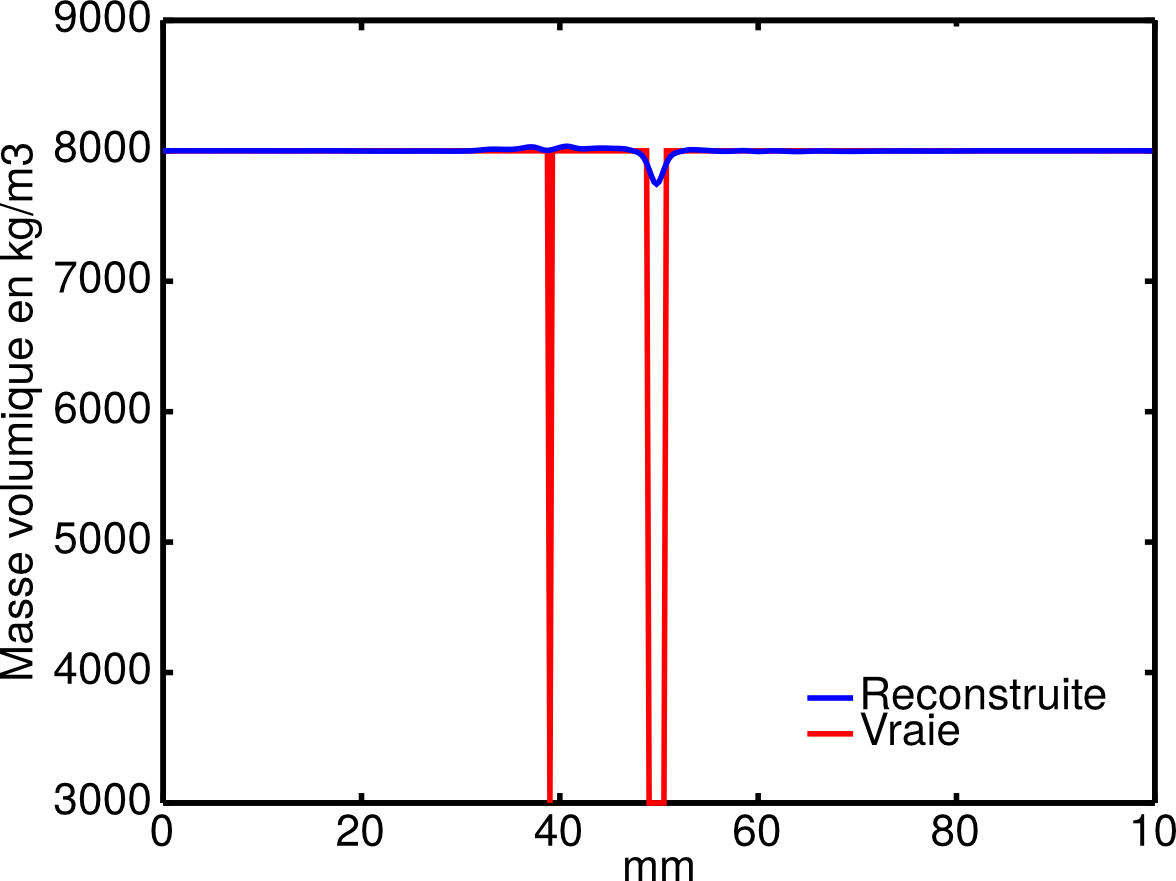
\includegraphics[width=\textwidth]{img/mono_param/coupe_rho_mono.png}
			\caption{Masse volumiques vraie et reconstruite à 3 cm de profondeur.}
		\end{subfigure}
		\caption{\label{app:inv_mono} Modèle initiaux et résultat d'inversion monoparamètre de la vitesse et de la densité.}
			\end{changemargin}
	\end{figure}




\subsubsection{Inversion multiparamètre}



multi paramètre  : c'est dur de savoir ce qui doit être interprété en vitesse et ce qui doit l'être en densité. Le risque est donc qu'une part de l'information soit attribuée à un paramètre alors qu'elle est induite par un autre paramètre. Il vaut donc mieux inverser la paramètre dominant dans les données : ici c'est vp, par son influence sur la cinématique et parce que rho ne change pas beaucoup dans la soudure et est plutôt HF (que au niveau des défauts). La stratégie est donc d'inverser la vitesse seule dans un premier temps pour construire un bon modèle de vitesse qui explique les arrivées puis inverser vp+rho (ou que rho ?) (au moment où on voit le défaut arriver ?)
stratégie : inverser vp avec fort smoothing pour n'expliquer que la cinématique en premier.
le but : voir si on améliore vp et info complémentaire pour la caractérisation donnée par rho ?


\begin{figure}[!h]
	\centering
	\begin{subfigure}[b]{0.45\textwidth}
		\includegraphics[width=\textwidth]{img/multi_param/vp_smooth.png}
		\caption{Modèle initial de vitesse.}
	\end{subfigure}\\
%	\begin{subfigure}[b]{0.45\textwidth}
%		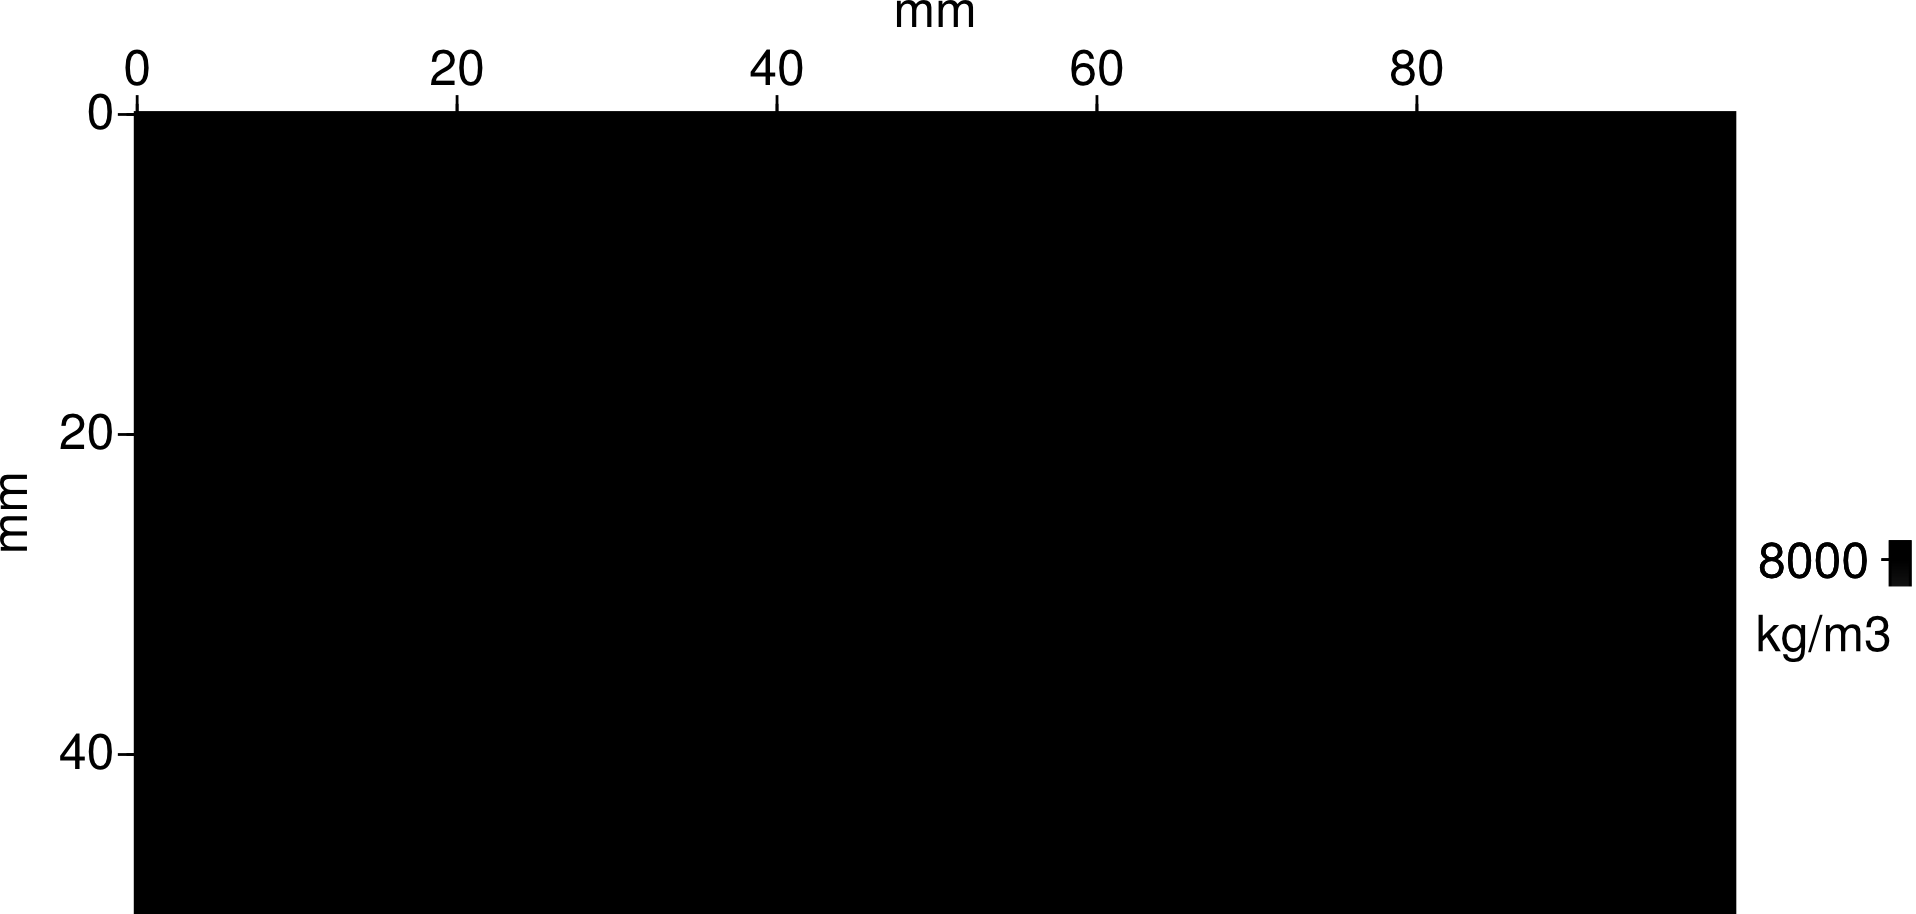
\includegraphics[width=\textwidth]{img/multi_param/rho_init.png}
%		\caption{}
%	\end{subfigure}
	\begin{subfigure}[b]{0.45\textwidth}
		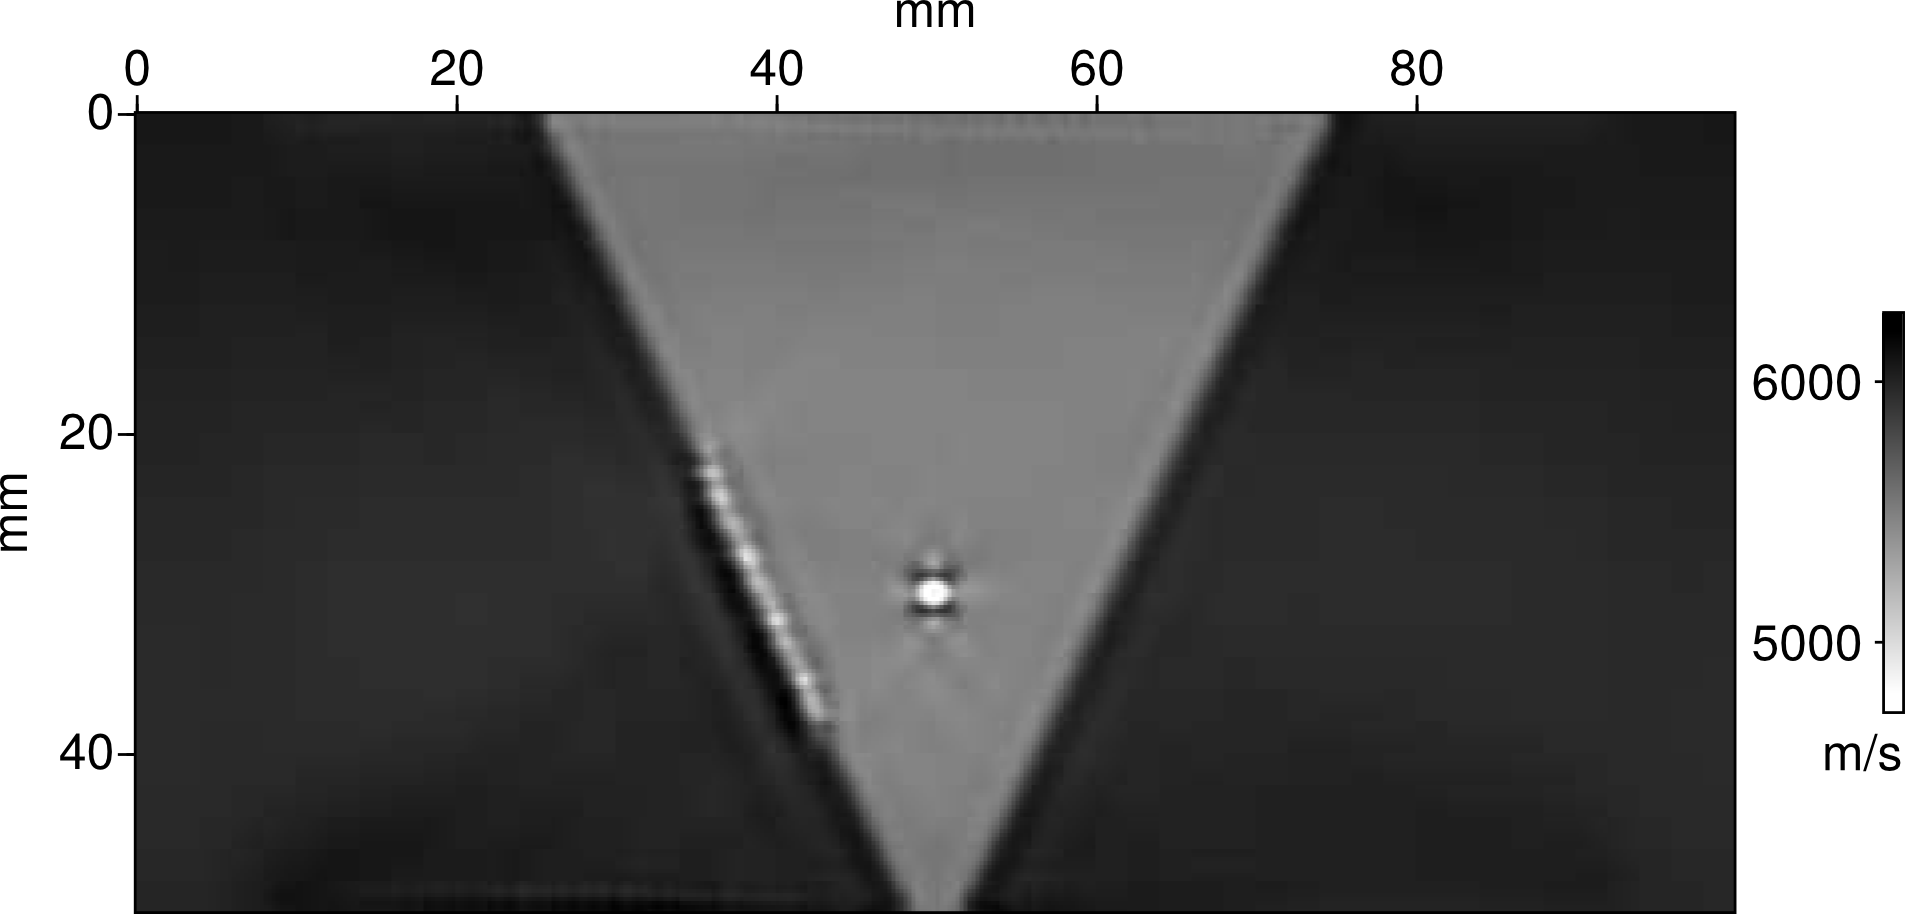
\includegraphics[width=\textwidth]{img/multi_param/vp_multi_6000k.png}
		\caption{Modèle final de vitesse obtenu par FWI multiparamètre.}
	\end{subfigure}
	\begin{subfigure}[b]{0.45\textwidth}
		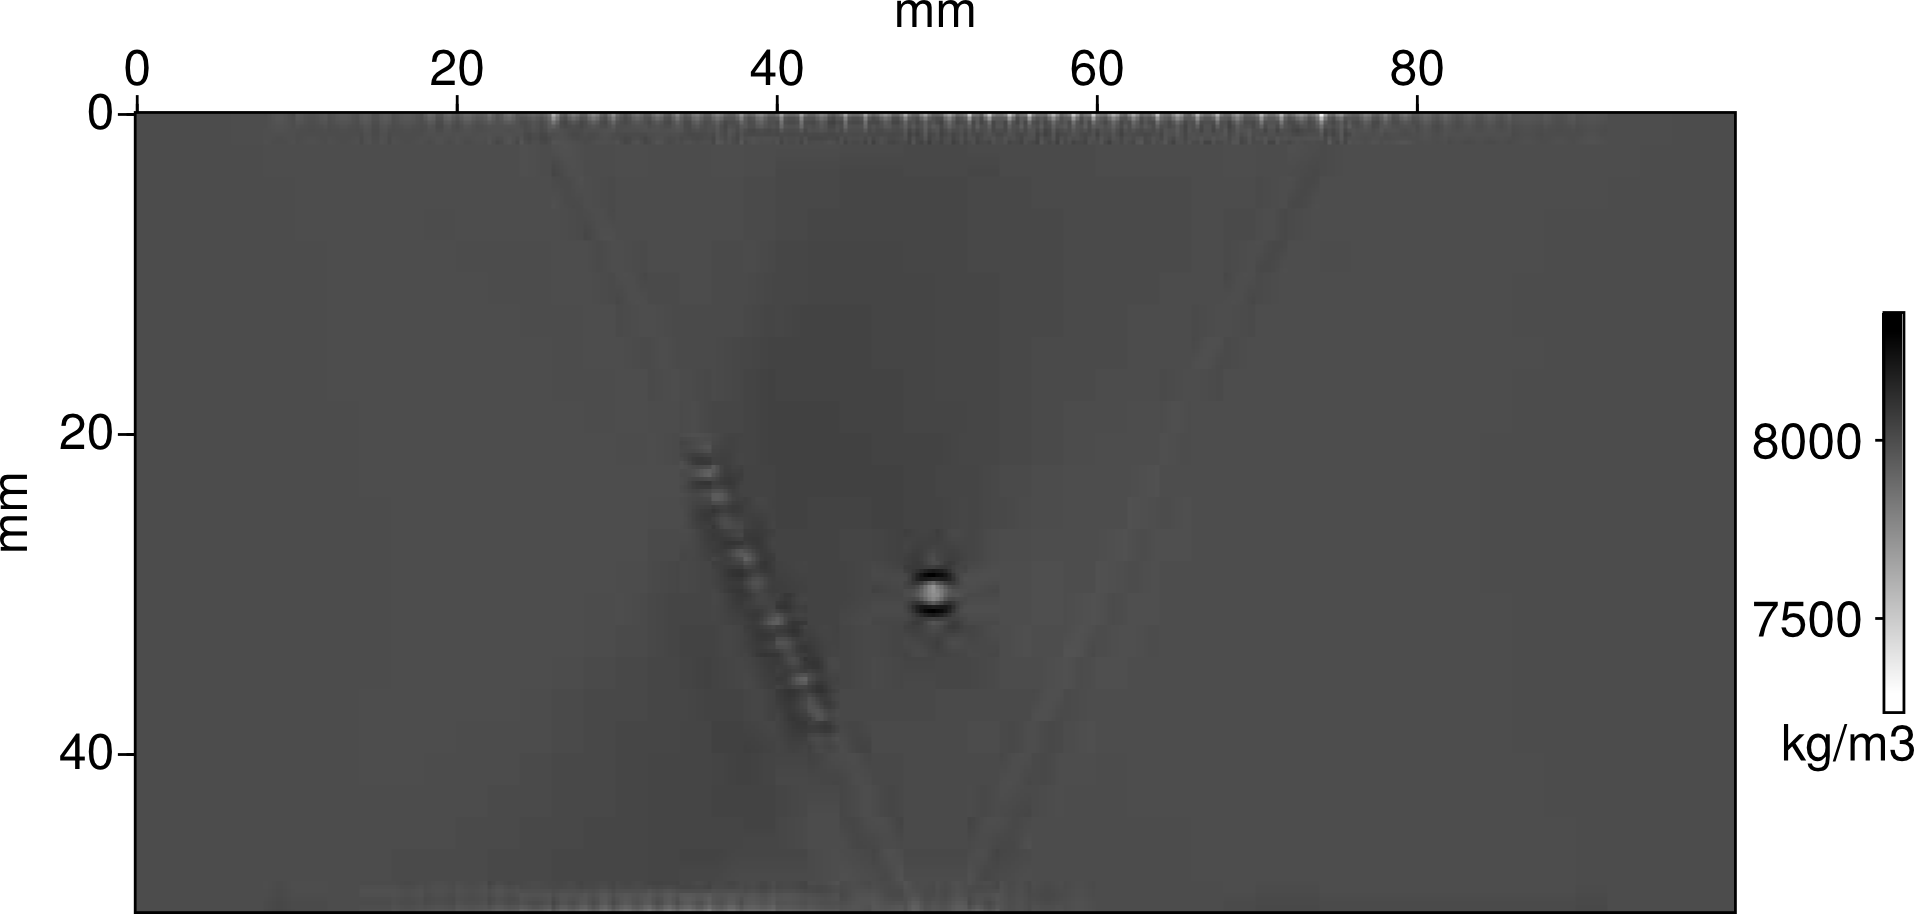
\includegraphics[width=\textwidth]{img/multi_param/rho_6000k.png}
		\caption{Modèle final de densité obtenu par FWI multiparamètre.}
	\end{subfigure}
	\begin{subfigure}[b]{0.45\textwidth}
		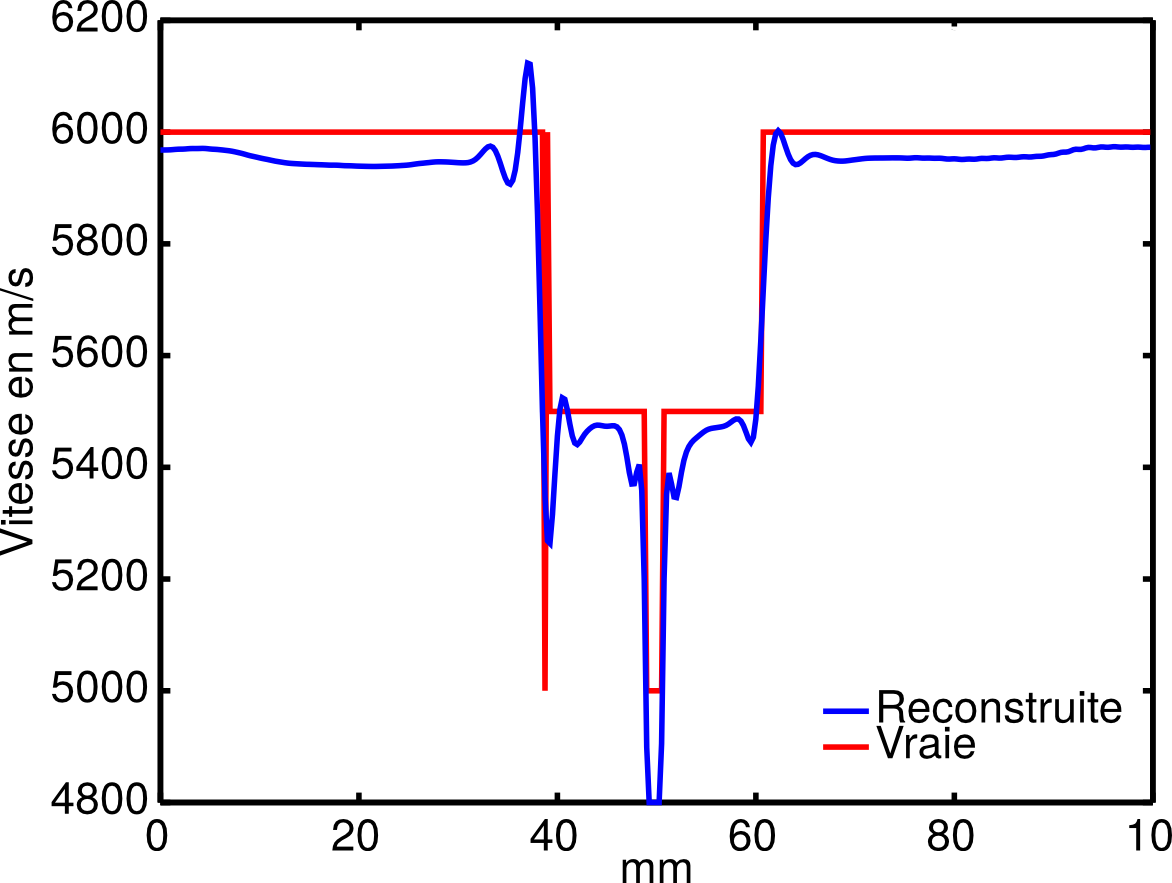
\includegraphics[width=\textwidth]{img/multi_param/coupe_vp_multi.png}
		\caption{Vitesses vraie et vitesse reconstruite à 3 cm de profondeur.}
	\end{subfigure}
	\begin{subfigure}[b]{0.45\textwidth}
		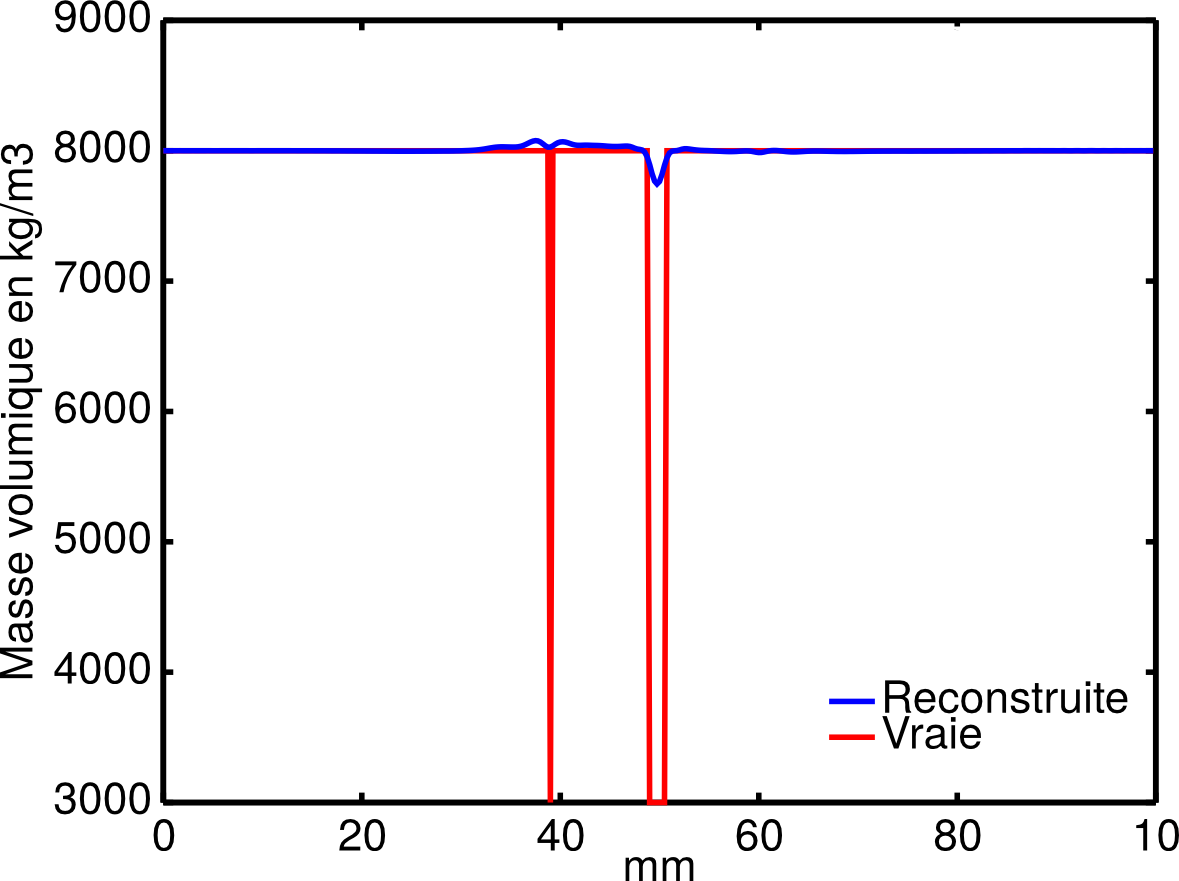
\includegraphics[width=\textwidth]{img/multi_param/coupe_rho_multi.png}
		\caption{Masse volumiques vraie et reconstruite à 3 cm de profondeur.}
	\end{subfigure}
	\caption{\label{app:inv_multi} }
\end{figure}


conclusion partielle : le multiparam, ça change rien à part que c'est plus dur et qu'il faut u meilleur modèle initial. La meilleure stratégie si on veut rho (qui peut donner des info pour la caractérisation du défaut) : inverser vp en mono, puis inverser rho en mono avec modèle vitesse initial venant de l'inversion




\subsection{Transverse isotrope}

Il est possible de formuler à partir de~\ref{prop} des équations d'ondes acoustiques en milieu anisotrope. Bien que ce soit physiquement impossible, cette formulation permet de se rapprocher cinématiquement des équations d'ondes élastiques, de manière simplifiée \citep{alkhalifah}.

Notons que cette formulation [Pose quelques problèmes (Duveneck 2008) notamment génération d'onde S (sur données "vrai simulée"  et sur problème direct, mais pas la même car différente grille, PML, ... donc on la mute sur le résidu) qui n'a pas de sens physique. Proposer les solutions (taper Epsilon, en sismo on est dans l'eau donc c'est fait naturellement -> placer les sources dans un milieu isotrope).]
 

La paramétrisation du milieu est faite à l'aide des constantes de Thomsen~\citep{thomsen} surtout utilisées dans le domaine des Sciences de la Terre définies comme suit : 
\begin{eqnarray}
	\epsilon & =  & \frac{C_{11}-C_{33}}{2C_{33}} = \frac{\bm{v}_{p}.\bm{e}_{x} -  \bm{v}_{p}.\bm{e}_{z}}{\bm{v}_{p}.\bm{e}_{z}}\\
	\delta & = & \frac{(C_{13}+C_{44})^2-(C_{33}-C_{44})^2}{2C_{33}(C_{33-C_{44}})}\text{.}\\
\end{eqnarray}
+theta

Le paramètre $\epsilon$ est donc lié à la différence entre la composante verticale et la composante horizontale de la vitesse des onde de pression et $\delta$ décrit davantage la propagation des ondes quasi-longitudinales.






\subsection{VTI}
Afin d'introduire une anisotropie simplifiée dans la soudure, une étude dans un milieu acoustique VTI est menée.\\

On considère une plaque isotrope dans laquelle se trouve une soudure anisotrope VTI sans défaut. On cherche à évaluer l'influence de l'anisotropie en vue d'inverser le paramètre $\epsilon$. La valeur de $\epsilon$ dans la soudure est fixée à 20\%, ce qui est environ deux fois plus élevé que les valeurs que l'on peut trouver dans la littérature~\citep{chassignole}. Les deux barrettes excitatrices/réceptrices sont placées de manière éloignée, afin d'accentuer la propagation des ondes suivant $\bm{e}_{x}$ et de s'assurer que les temps de vol soient perturbés par l'anisotropie (figure~\ref{configuration_vti}).\\
Les autres paramètres ($v_{p}$,$\rho$ et $\delta$) sont supposés constants et uniformes.\\

Une comparaison des données observées en milieu isotrope ($\epsilon = 0$) et avec la soudure anisotrope est proposée en figure~\ref{}. Il apparaît que la présence d'une anisotropie VTI a peu d'impact sur les données, car le dispositif d'acquisition favorise la mesure des ondes dont le trajet est majoritairement vertical et donc peu perturbé.\\
 L'inversion du paramètre $\epsilon$ est alors difficile : une modification grossière de la vitesse horizontale suffit à corriger les retards résiduels (cf figure~\ref{}).
 
 \todo[inline]{figures : configurations ; traces isotrope, epsilon=20 ; inversion + données calculées}
 
Un modèle de soudure anisotrope VTI est donc trop simple pour représenter l'anisotropie d'une soudure réelle, dont on sait qu'elle impacte beaucoup le faisceau ultrasonore. Pour tester la capacité de la FWI à reconstruire ces paramètres d'anisotropie, il est donc nécessaire d'utiliser un modèle plus pertinent qui se rapprocherait davantage de celui proposé par \cite{ogilvy} par exemple.\\

Le modèle proposé par \cite{ogilvy} est de la forme : 
\begin{equation}
	\theta(x,z) = \tan^{-1}\left( \frac{D/2 + z\tan\alpha}{x} \right),
\end{equation}
avec $D$ la largeur de la racine de la soudure et $\alpha$  l'angle du bord de soudure.

 Conclusion : inversion de $\epsilon$ -> dur et par pertinent
passer en tilted (façon ogilvy ?) ou modèle plus précis en élastique.






\section{Inversions en matériau élastique isotrope}




%%%%%%%%%%%%%%%%%%%%%notes%%%%%%%%%%%%%%%
\todo[inline]{notes : }
\subsection{anisotrope}

anisotrope est plus problématique que isotrope car : 
-modélisation plus complexe,
-problème moins bien posé

Gholami 2011 : la vitesse a beaucoup plus d'influence sur les données que les paramètres delta et epsilon (delta étant le plus faible). D'après ses schémas, on va donc avoir une maj de la vitesse mais pas des autres paramètres

modèle initial de soudure : citer mina ?

%VTI elliptique ne gène pas l'inversion car beaucoup d'info portées par la transmission (vecteurs d'ondes verticaux non affectés par l'anisotropie elliptique VTI)  -> pas assez proche du modèle réel

%le flop du vti montre que l'inversion des paramètres est tributaire de l'acquisition

Romain : passer en TTI (code en freq)

